\chapter{Resultados}
Com a técnica de geração procedural de terrenos proposta neste trabalho é possível criar uma 
malha de triângulos para desenhar o terreno. A abordagem é procedural, sem nenhuma 
intervenção humana, os resultados apresentam regiões para diferentes aspectos de terrenos,
os biomas, o algoritmo proposto é capaz de deixar as fronteiras entre esses com características 
contínuas, tendo uma transição gradual e linear entre os biomas.

Cada bioma tem seus parâmetros para o ruído de \textit{perlin}, que são as oitavas ($\theta$)
e a frequência ($f$). O 'deserto' e a 'planície' possuem aparências mais onduladas, portanto, têm
um valor menor em $\theta$. Além dos parâmetros do ruído, a maneira com que cada 
bioma usa o retorno gerado por essa função ($h'$) também é diferente. Esse valor de retorno
é usado para calcular a cor e cada bioma possui três cores para escolher como fazer o cálculo de interpolação, as cores obtidas se referem às alturas mais elevadas, medianas e baixas. Outro uso do $h'$
é como parâmetro para decidir a altura e cada bioma tem uma maneira diferente de realizar
esse cálculo. A 'planície' e o 'deserto' apenas são multiplicadas $h'$ por um escalar, enquanto
'montanhas' usam exponenciais, já o 'deserto' utiliza \textit{clamp} em $h'$ para depois
usar um expoente. Os resultados de cada bioma podem ser vistos nas imagens \ref{fig:bssComBiomasFixados}.
O trabalho de definir o comportamento de cada bioma com os parâmetros apresentados 
é tanto quanto artístico, de nenhuma maneira este trabalho tenta fazer grandes aproximações
com os aspectos encontrados na natureza. A proposta aqui feita é mostrar como usar
a saída do ruído de Perlin para poder criar diferentes características em algum terreno, em 
seguida mostrar uma maneira procedural de separar estes biomas em regiões e criar fronteiras
entre biomas distintos de maneira contínua, mesmo com essa diferença de aspectos.

%\begin{figure}[H]
%    \centering
%    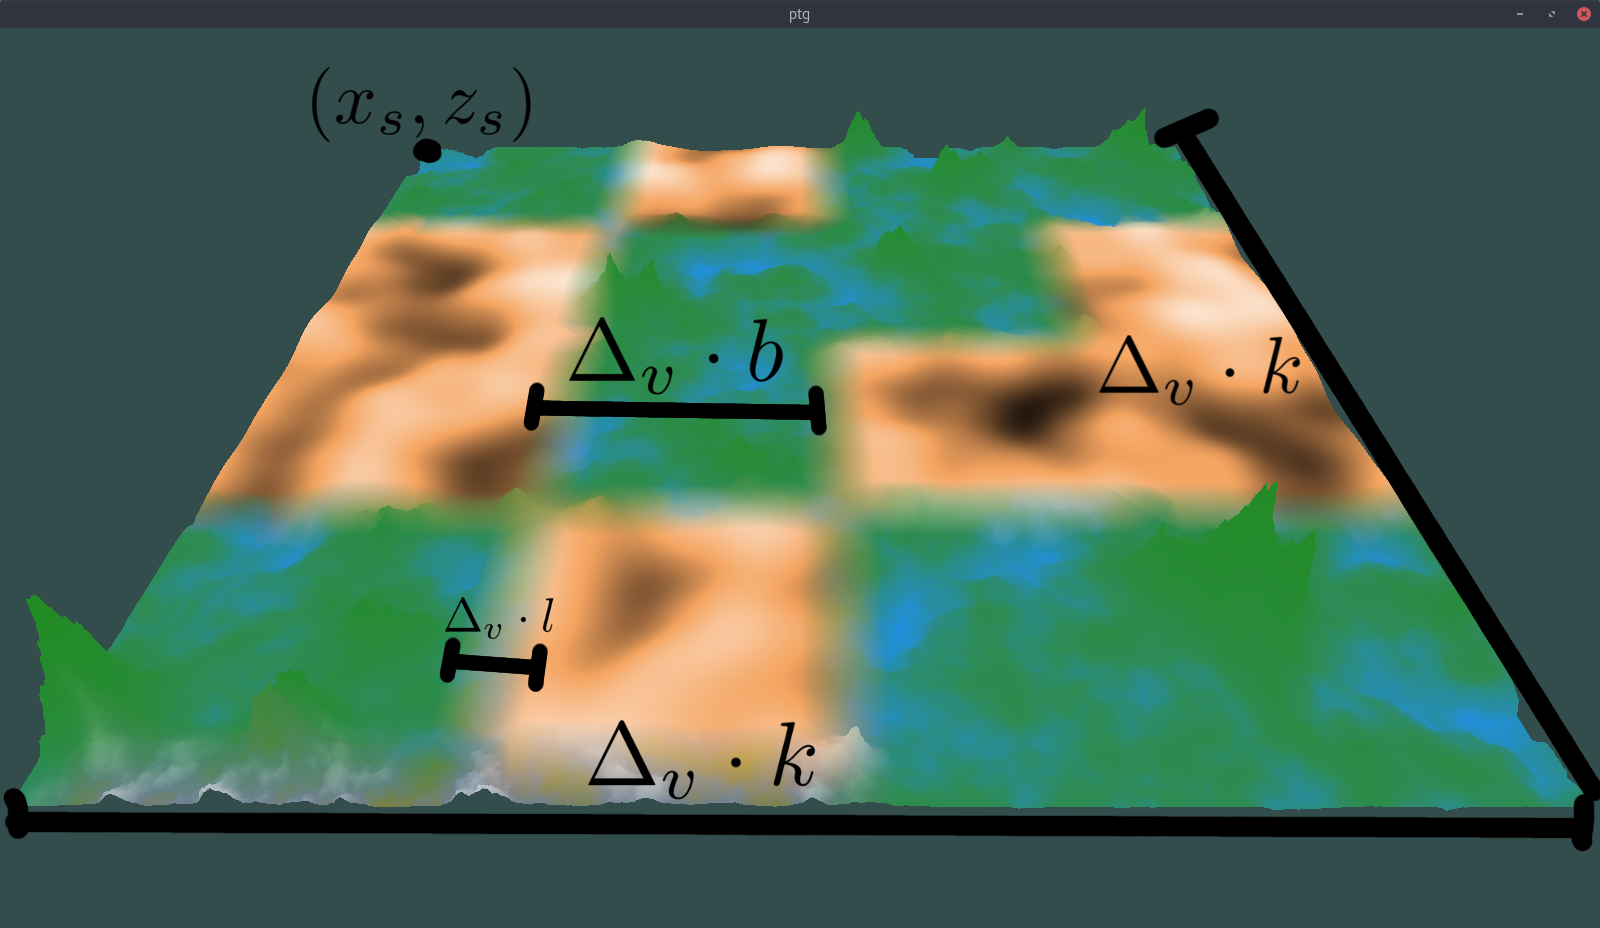
\includegraphics[width=0.75\textwidth]{figuras/resultados/sseditada.png}
%    \caption{sseditada}
%    \label{fig:sseditada}
%\end{figure}
\begin{figure}[H]
     \centering
     \subfloat[][$biomaTipo =$ Planícies]{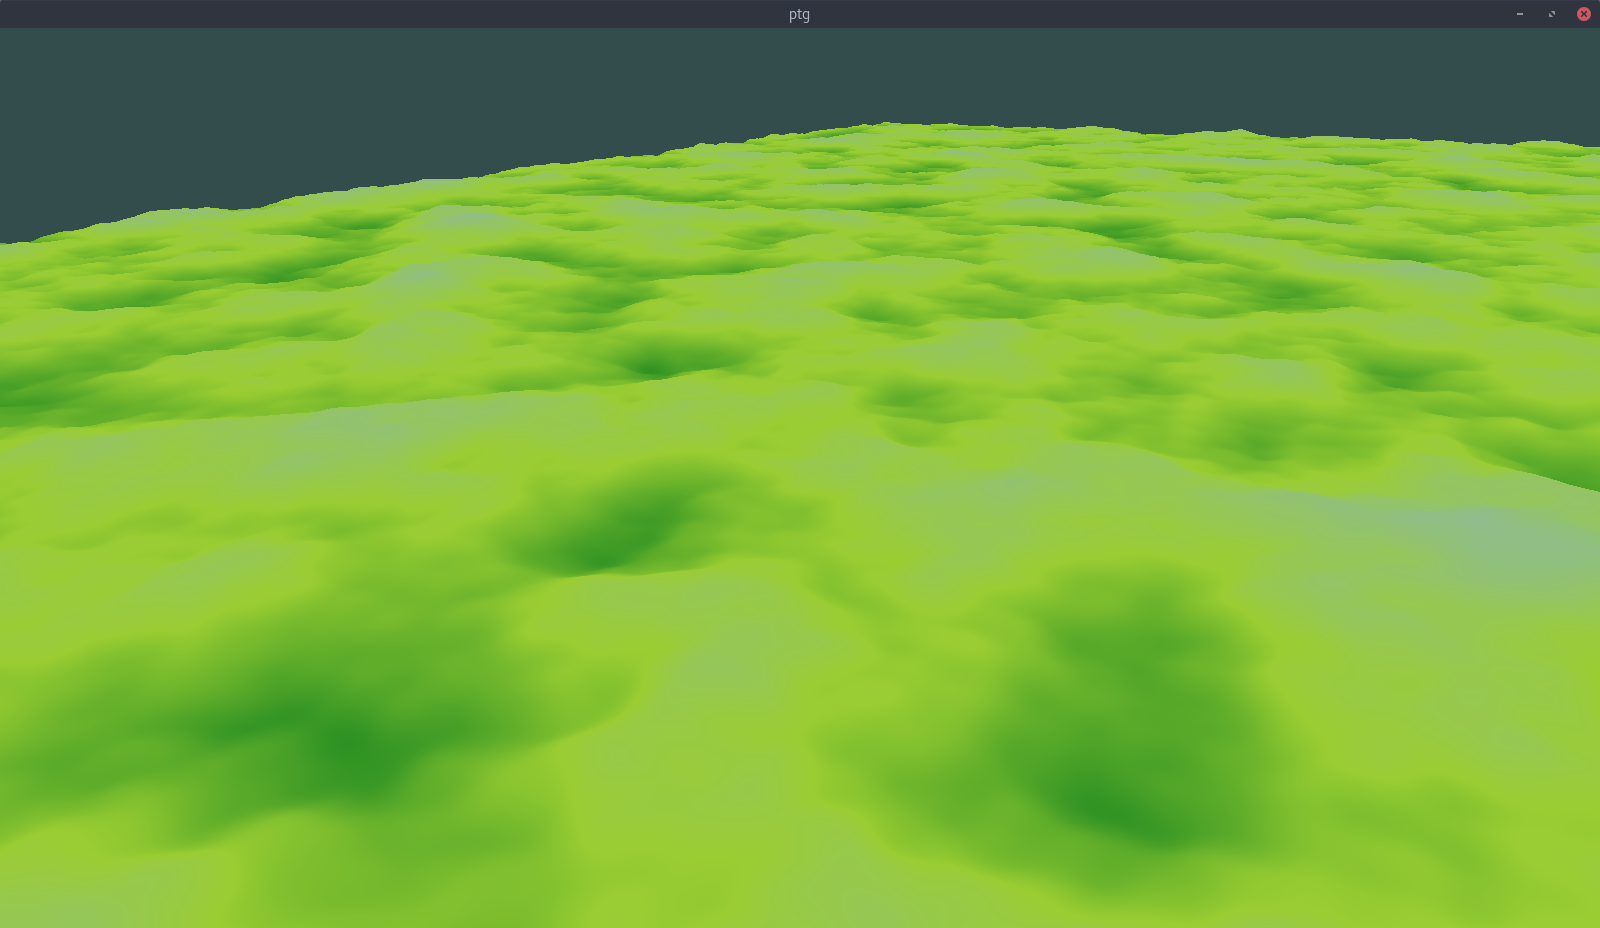
\includegraphics[width=0.48\textwidth]{figuras/bssPlains.png}\label{fig:biomaTipo1}}\hspace{0.1cm}
     \subfloat[][$biomaTipo =$ Montanhas]{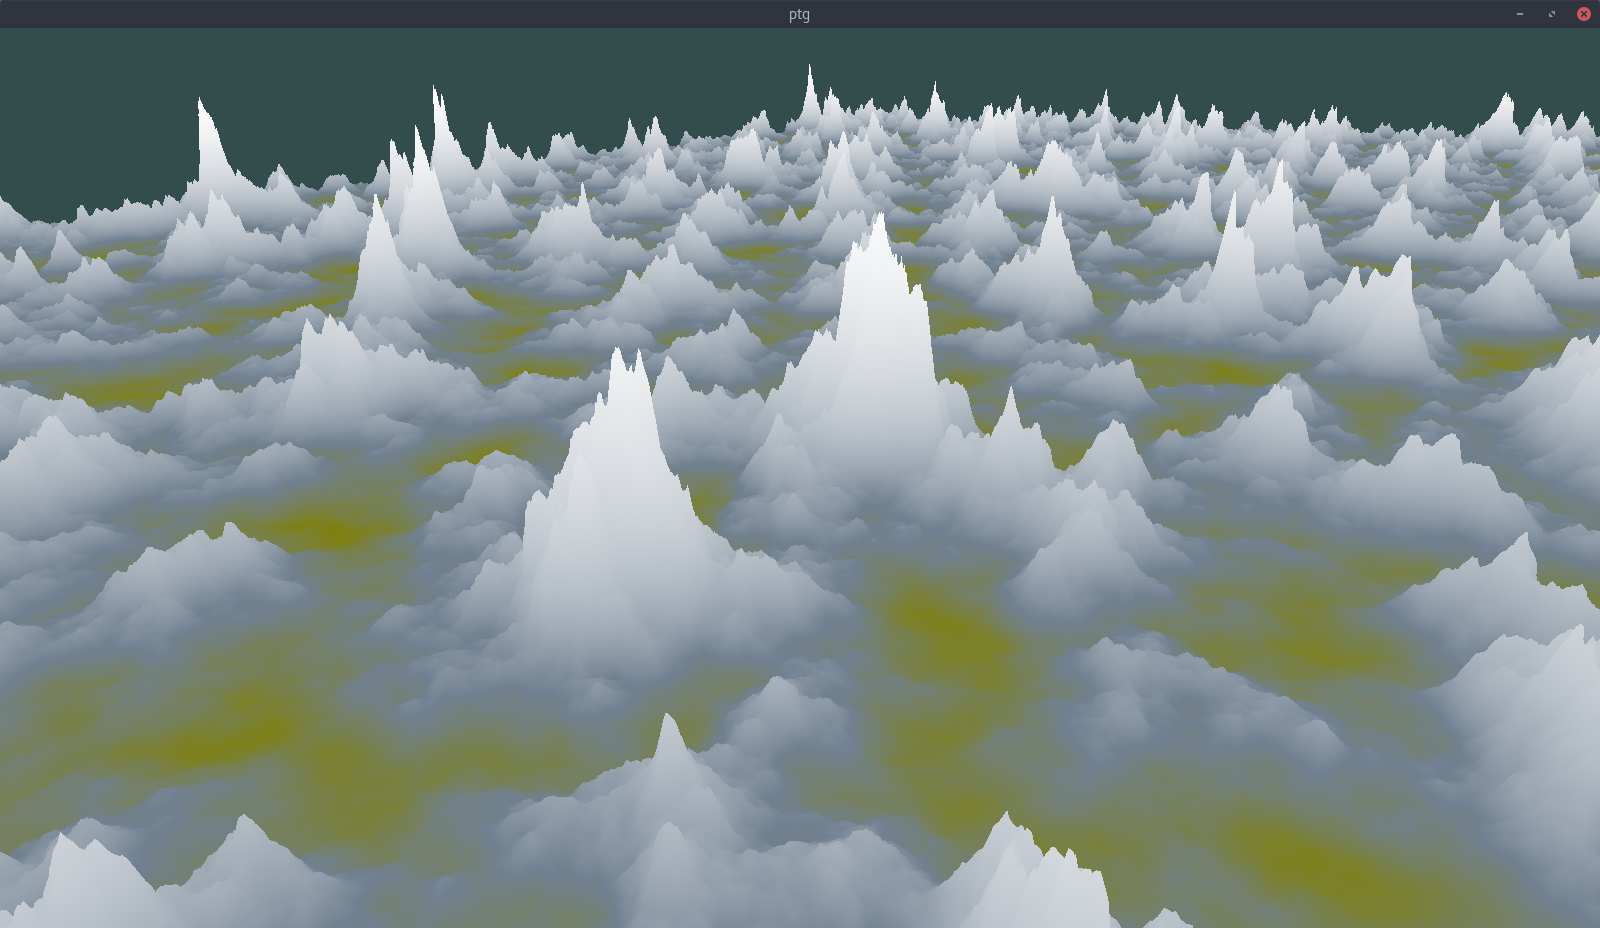
\includegraphics[width=0.48\textwidth]{figuras/bssMontains.png}\label{fig:biomaTipo2}}\\
     \subfloat[][$biomaTipo =$ Vales]{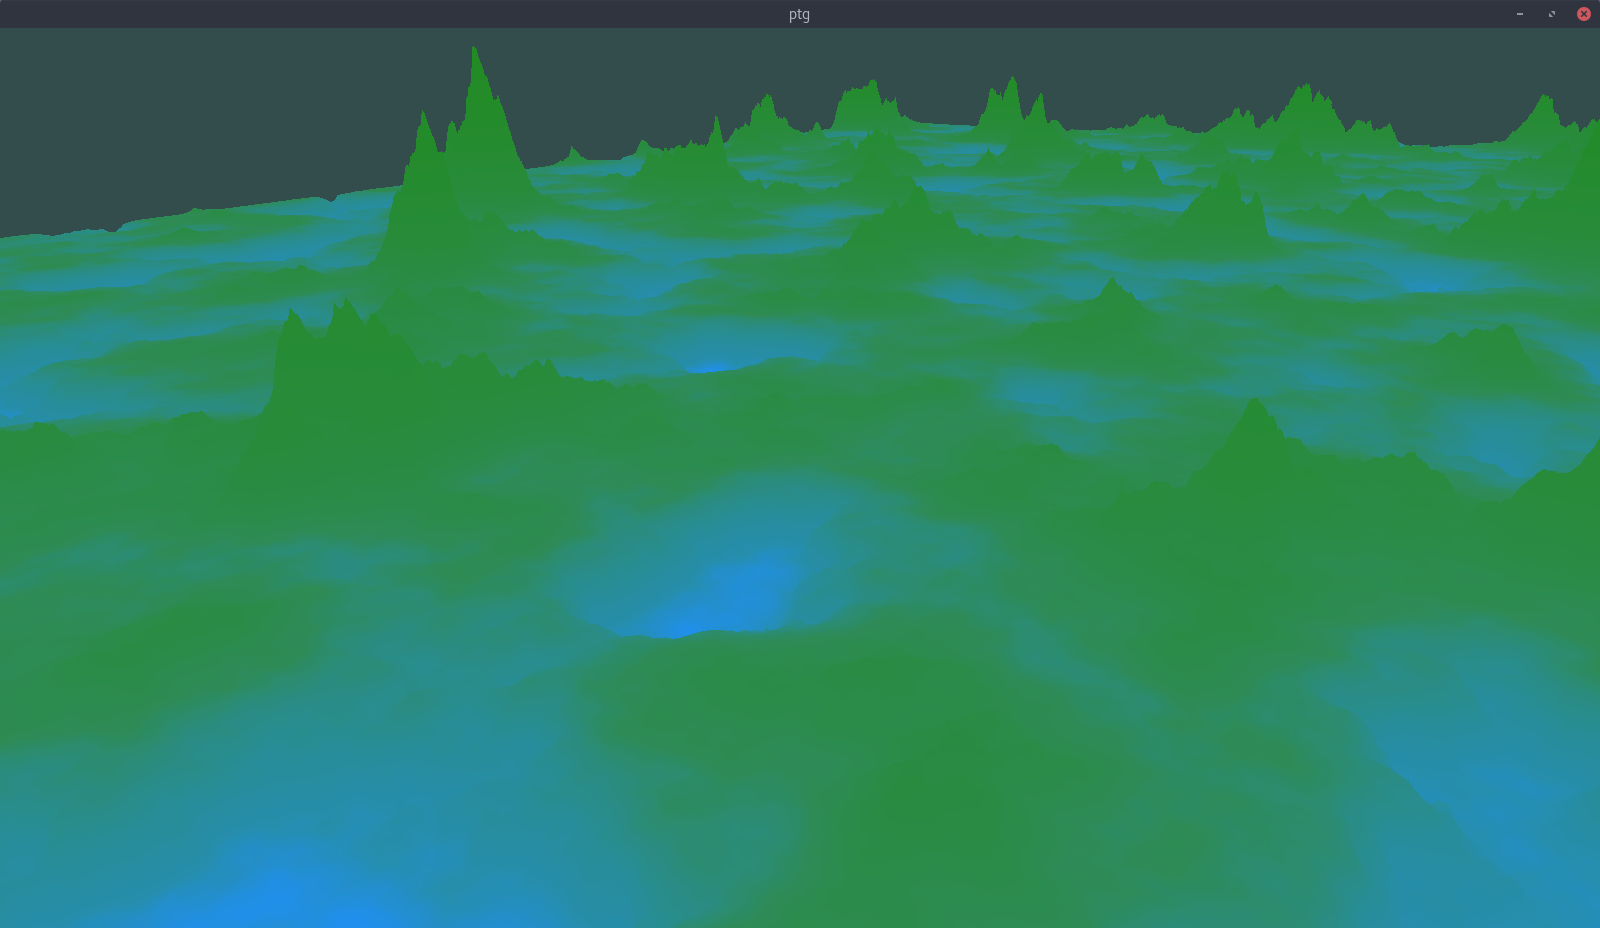
\includegraphics[width=0.48\textwidth]{figuras/bssValley.png}\label{fig:biomaTipo3}}\hspace{0.1cm}
     \subfloat[][$biomaTipo =$ Deserto]{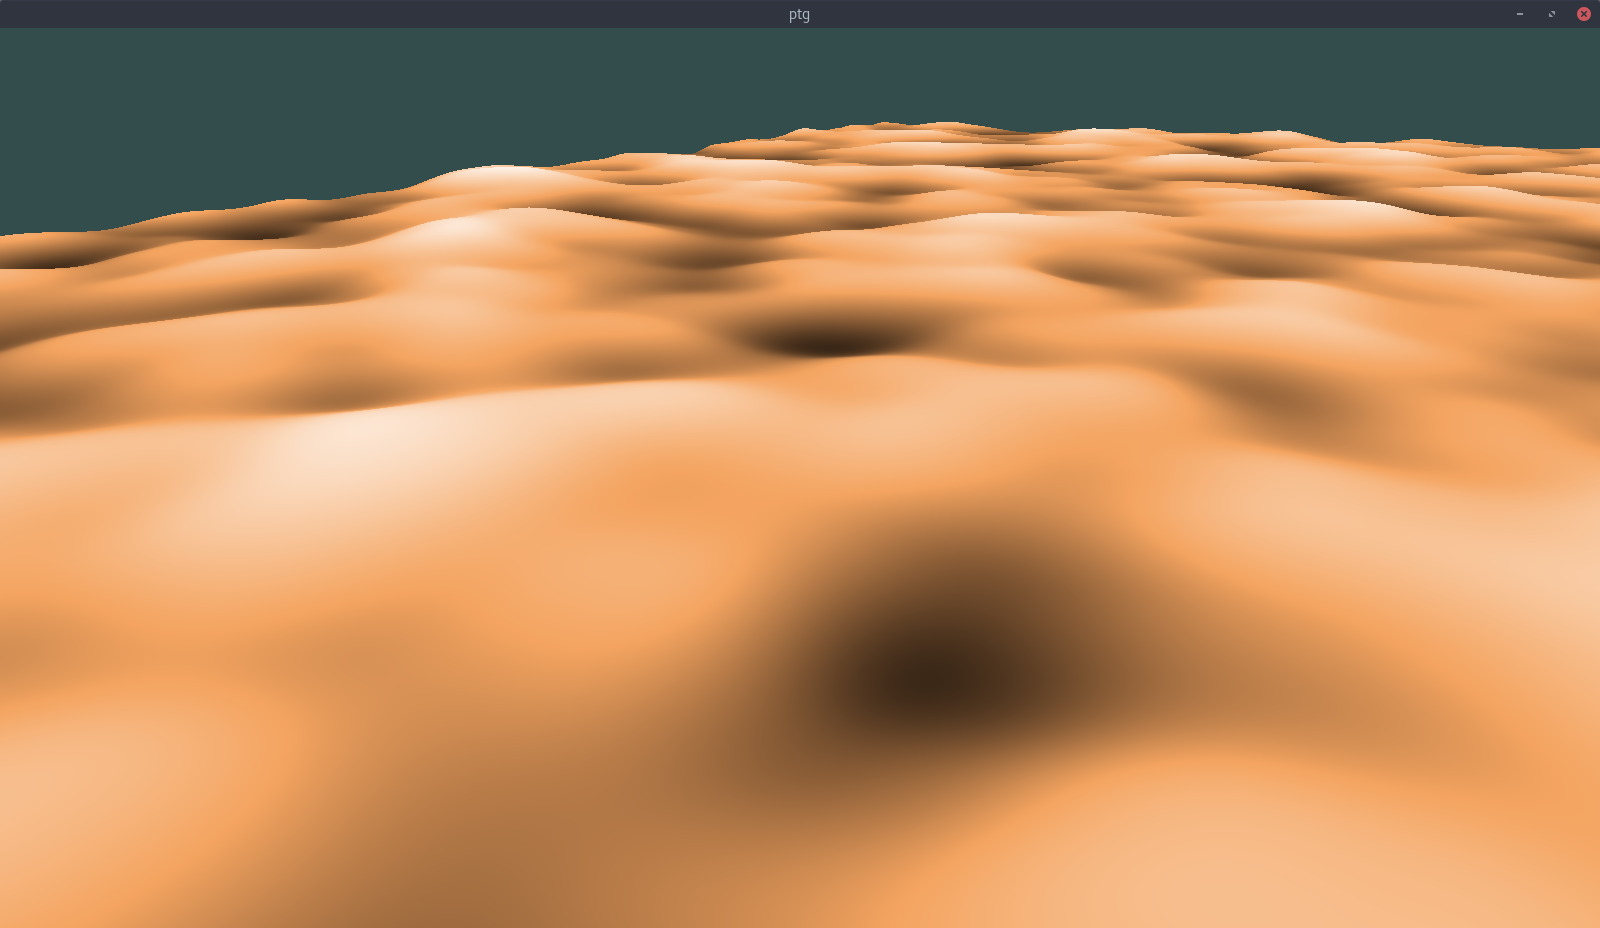
\includegraphics[width=0.48\textwidth]{figuras/bssDesert.png}\label{fig:biomaTipo4}}\\
     \subfloat[][$biomaTipo =$ Cânyons]{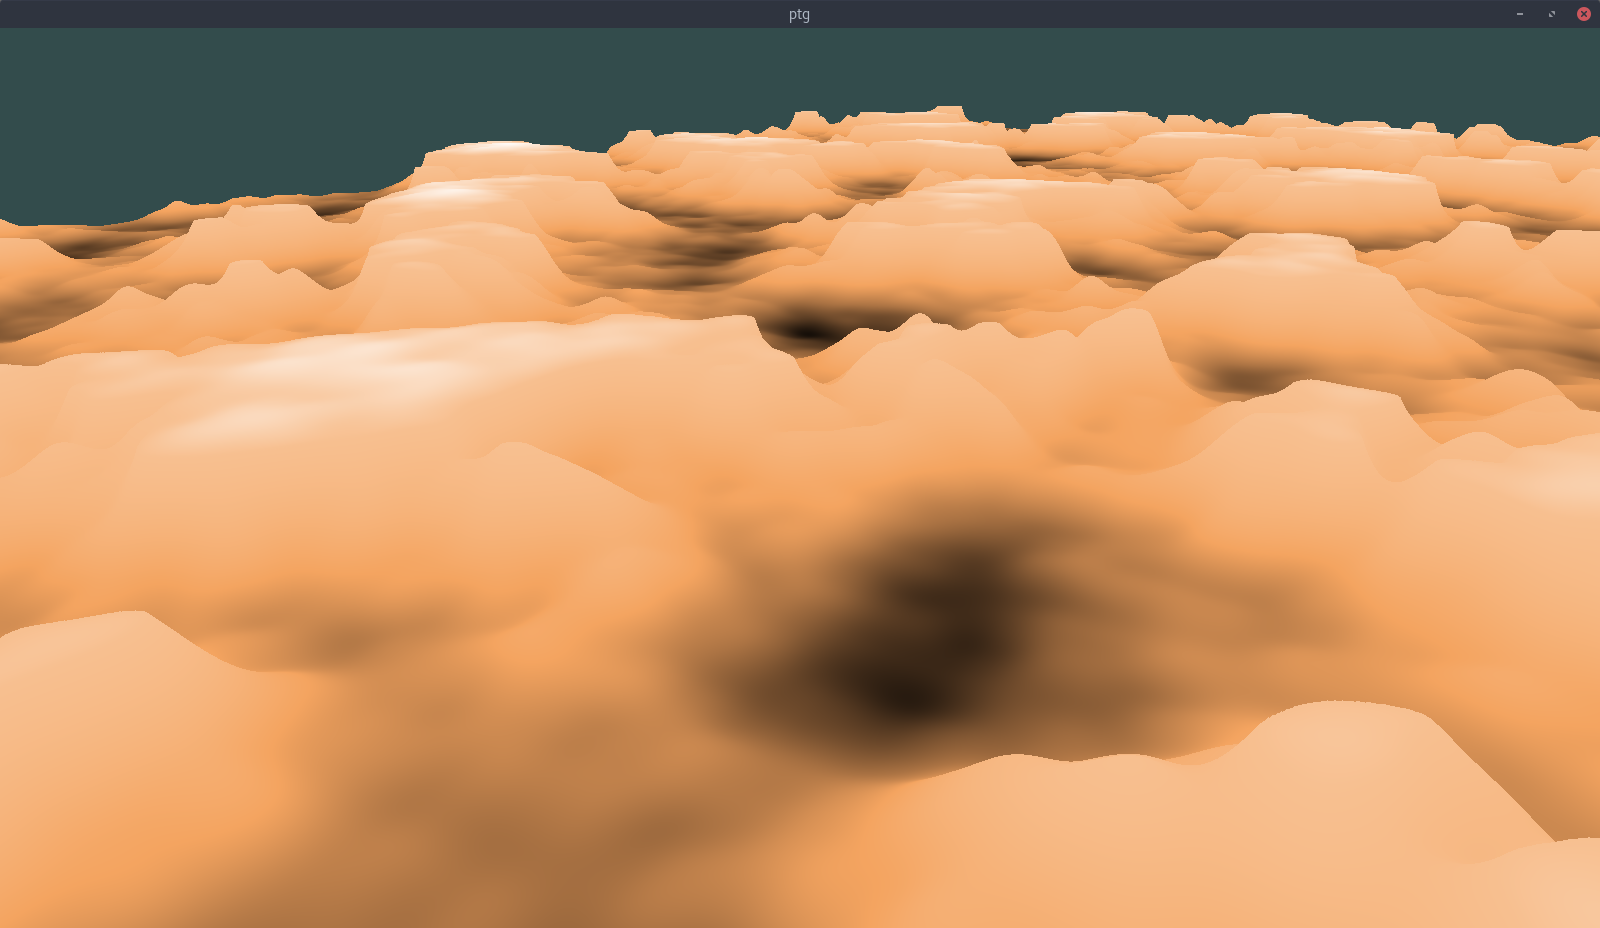
\includegraphics[width=0.48\textwidth]{figuras/bssCanyons.png}\label{fig:biomaTipo5}}
     
     \caption{Resultado dos Biomas fixados.}
     
     \label{fig:bssComBiomasFixados}
     % usar \hspace{0.1cm}, é gambiarra mas funciona
\end{figure}

As regiões dos biomas são separadas em áreas quadradas de proporção $b$, para definir
qual bioma pertence a cada área é usado o ruído, mas dessa vez a entrada se dá por valores
truncados da localização dividida por $b$ e temos o parâmetro $fb$ que define a frequência nas
mudanças de bioma. A influência destes parâmetros podem ser visualizados nas imagens \ref{fig:comparandoareadebiomasyeah} e \ref{fig:comparandofreqdebiomasyeah}.

Uma das vantagens de usar ruído para decidir qual bioma pertence a qual 
região é que ele matem próximo biomas de valores parecidos, neste trabalho a ordem de 
valores usados foi \{Planícies, Montanhas, Vales, Deserto e Cânyons\}, então temos as seguintes
características encontradas, 'planícies' e 'cânyons' estão nas extremidades, então eles 
tem ocorrências raras, 'planícies' costumam ser rodeados por montanhas, 'cânyons' costumam
ser rodeados por 'deserto', provavelmente terá a ocorrência de 'vales' entre 'montanhas' e 'desertos'.
Isso pode ser facilmente ser usado para desenvolver um jogo na hora de distribuir 
a raridade dos biomas e a probabilidade de proximidade entre eles, isso é visível em algumas das imagens \ref{fig:comparandofreqdebiomasyeah}.

\begin{figure}[H]
     \centering
     \subfloat[][$b = 16$]{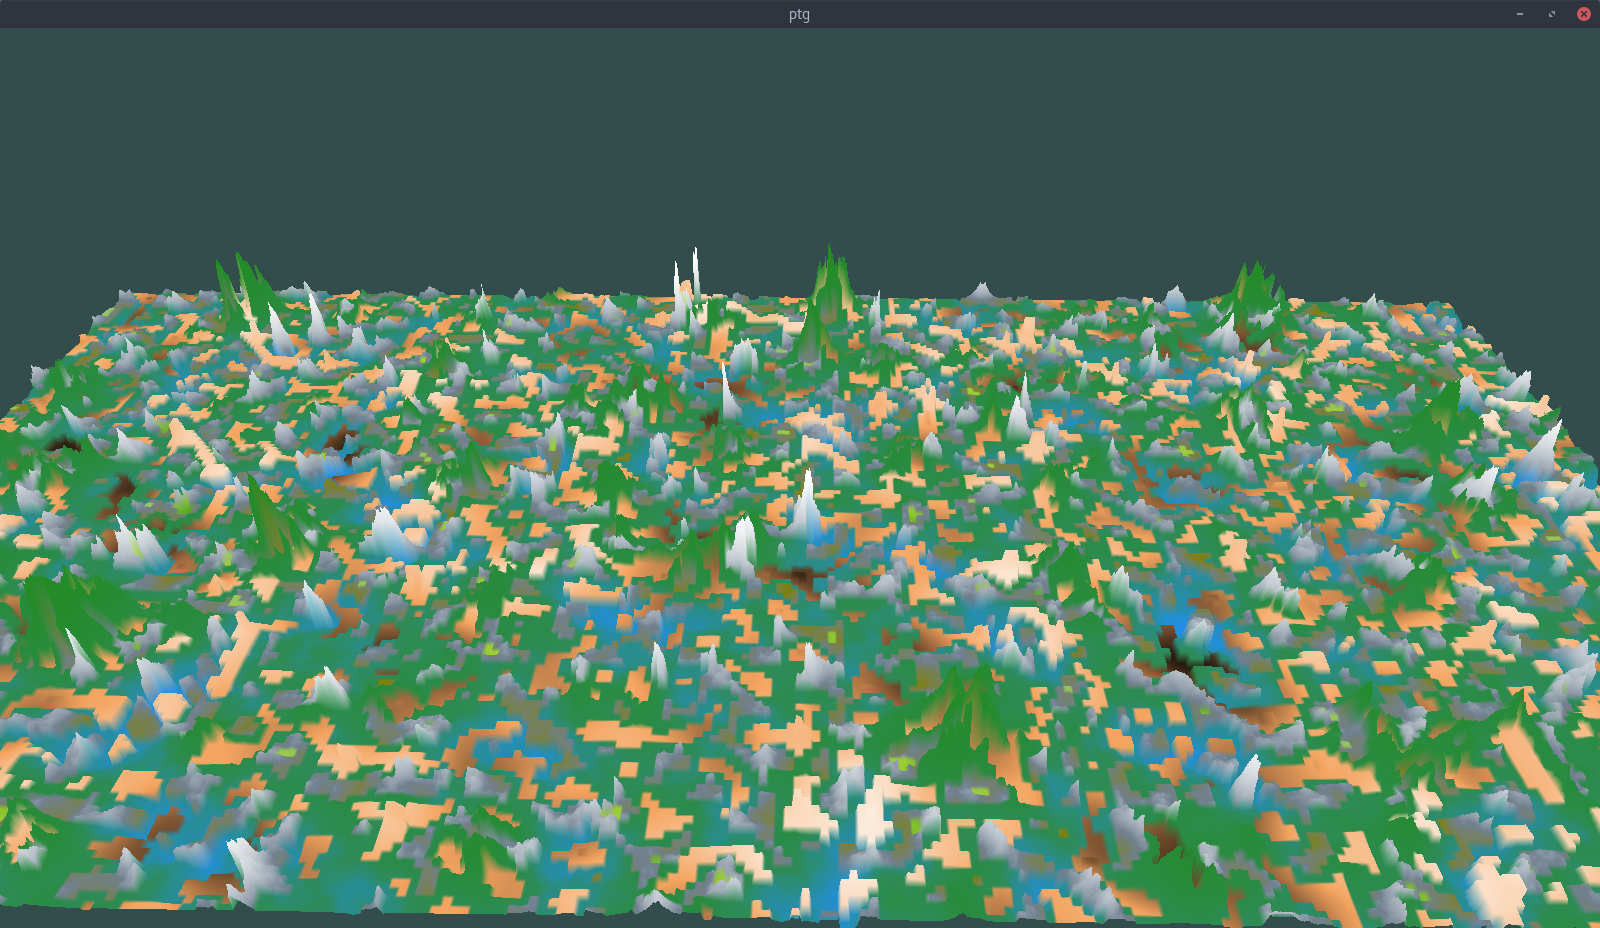
\includegraphics[width=0.31\textwidth]{figuras/re2bfb/b/16f4.png}\label{fig:re2bfb_b_16f4}}\hspace{0.1cm}
     \subfloat[][$b = 32$]{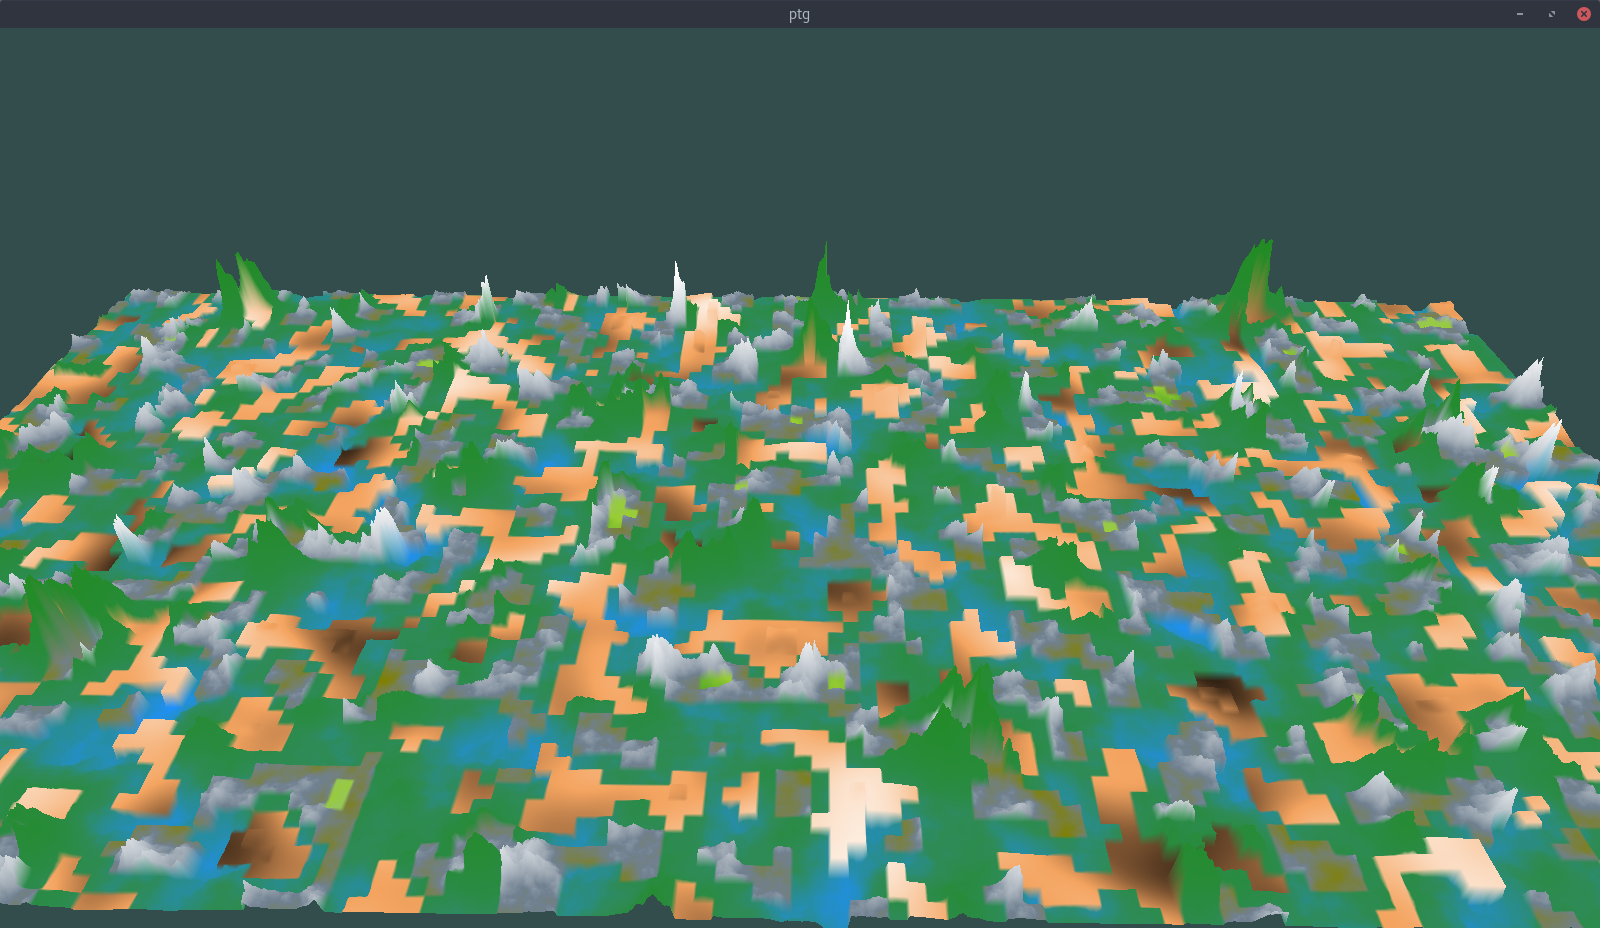
\includegraphics[width=0.31\textwidth]{figuras/re2bfb/b/32f4.png}\label{fig:re2bfb_b_32f4}}\hspace{0.1cm}
     \subfloat[][$b = 64$]{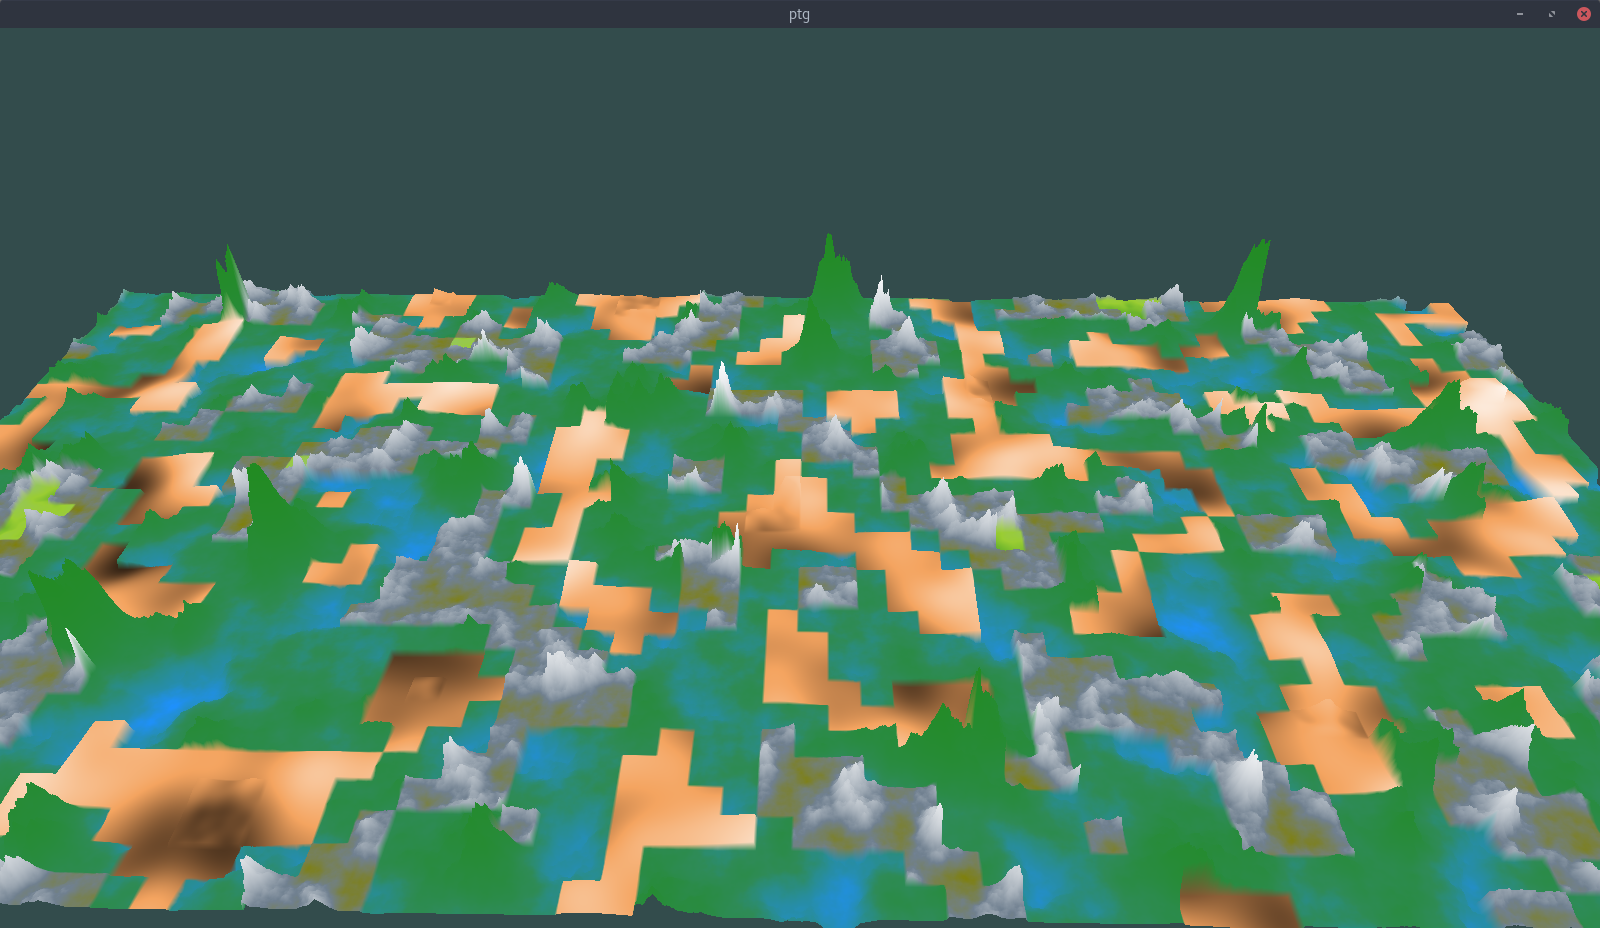
\includegraphics[width=0.31\textwidth]{figuras/re2bfb/b/64f4.png}\label{fig:re2bfb_b_64f4}}\\
     \subfloat[][$b = 128$]{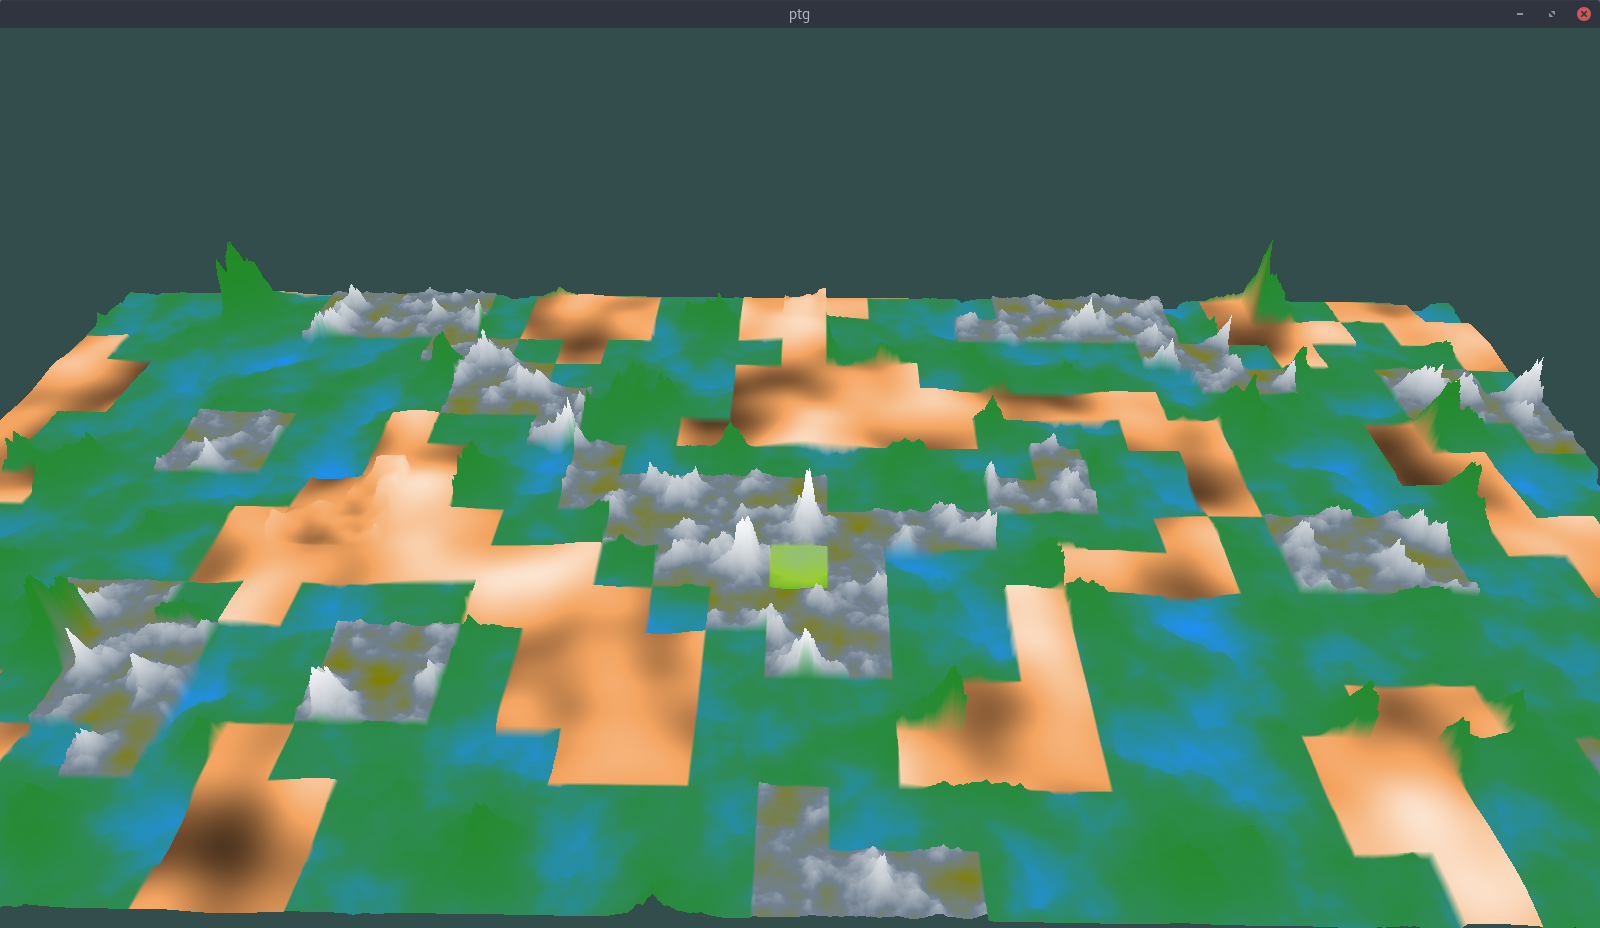
\includegraphics[width=0.31\textwidth]{figuras/re2bfb/b/128f4.png}\label{fig:re2bfb_b_128f4}}\hspace{0.1cm}
     \subfloat[][$b = 256$]{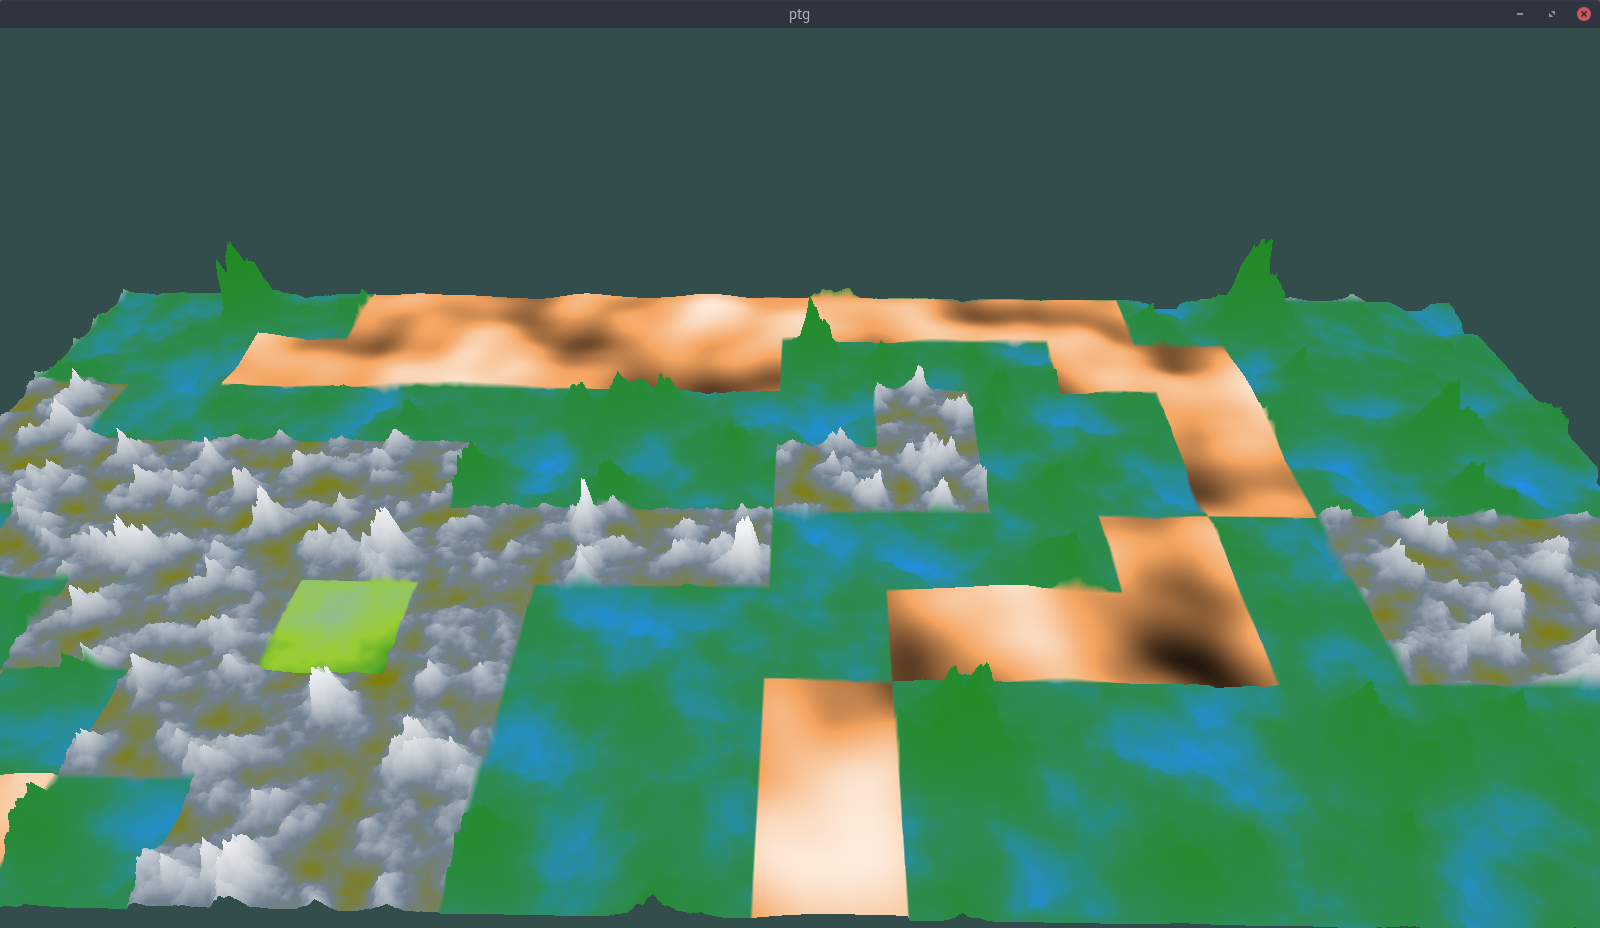
\includegraphics[width=0.31\textwidth]{figuras/re2bfb/b/256f4.png}\label{fig:re2bfb_b_256f4}}\hspace{0.1cm}
     \subfloat[][$b = 512$]{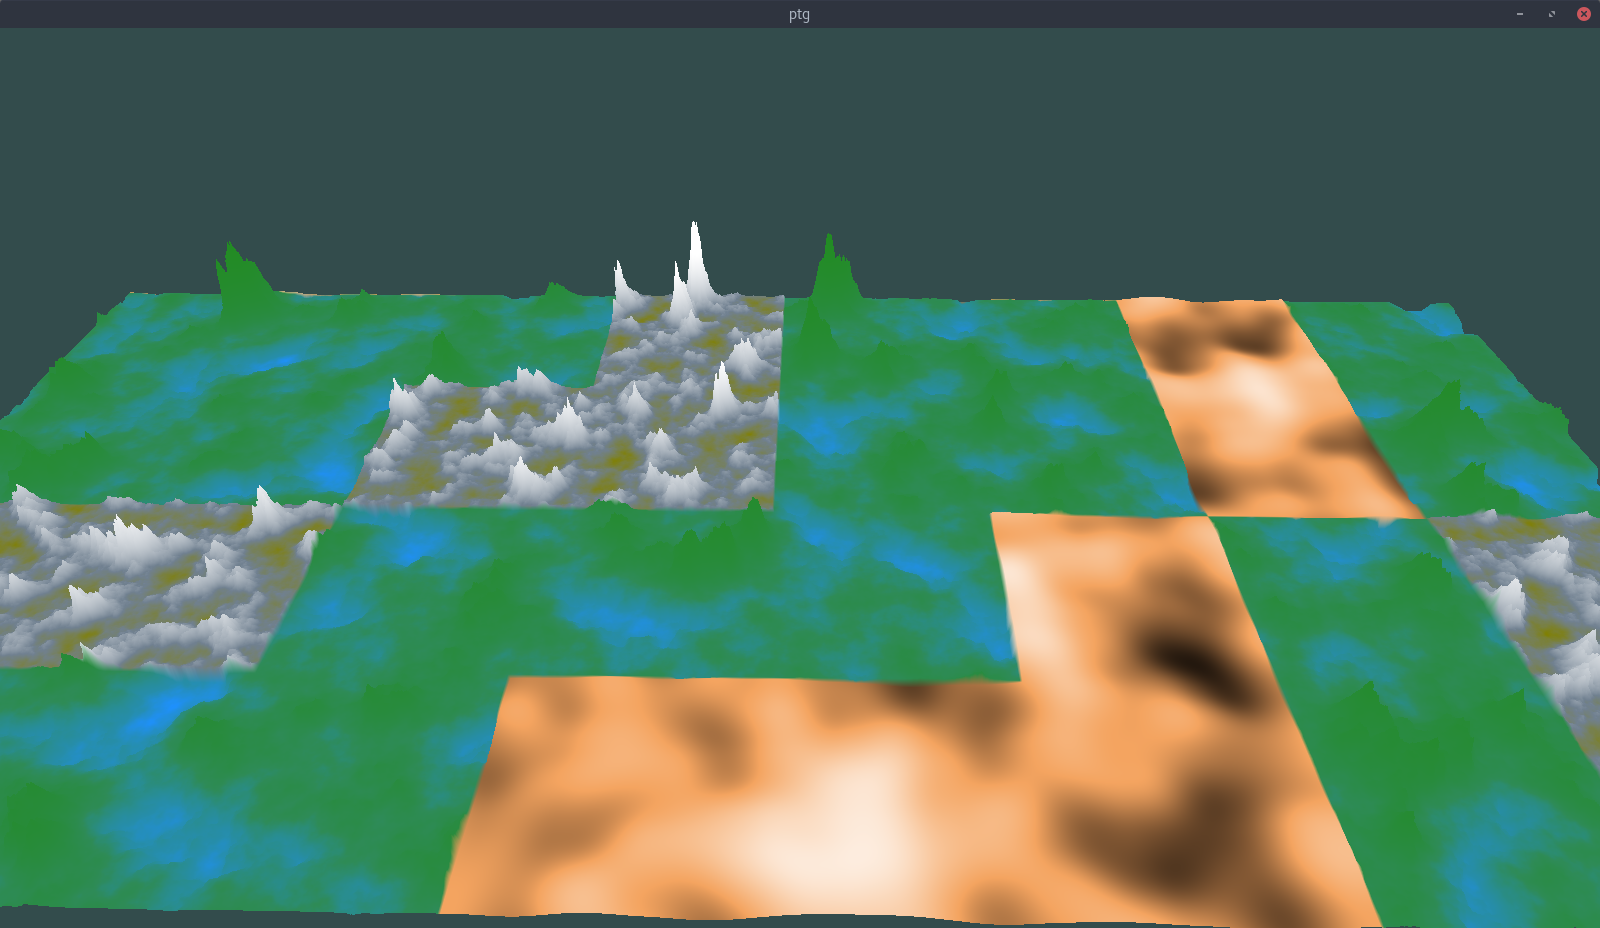
\includegraphics[width=0.31\textwidth]{figuras/re2bfb/b/512f4.png}\label{fig:re2bfb_b_512f4}}
     
     \caption{Diferentes tamanhos para áreas de bioma($b$), usando $fb = 4$.}
     
     \label{fig:comparandoareadebiomasyeah}
     % usar \hspace{0.1cm}, é gambiarra mas funciona
\end{figure}

\begin{figure}[H]
     \centering
     \subfloat[][$fb = 0.5$]{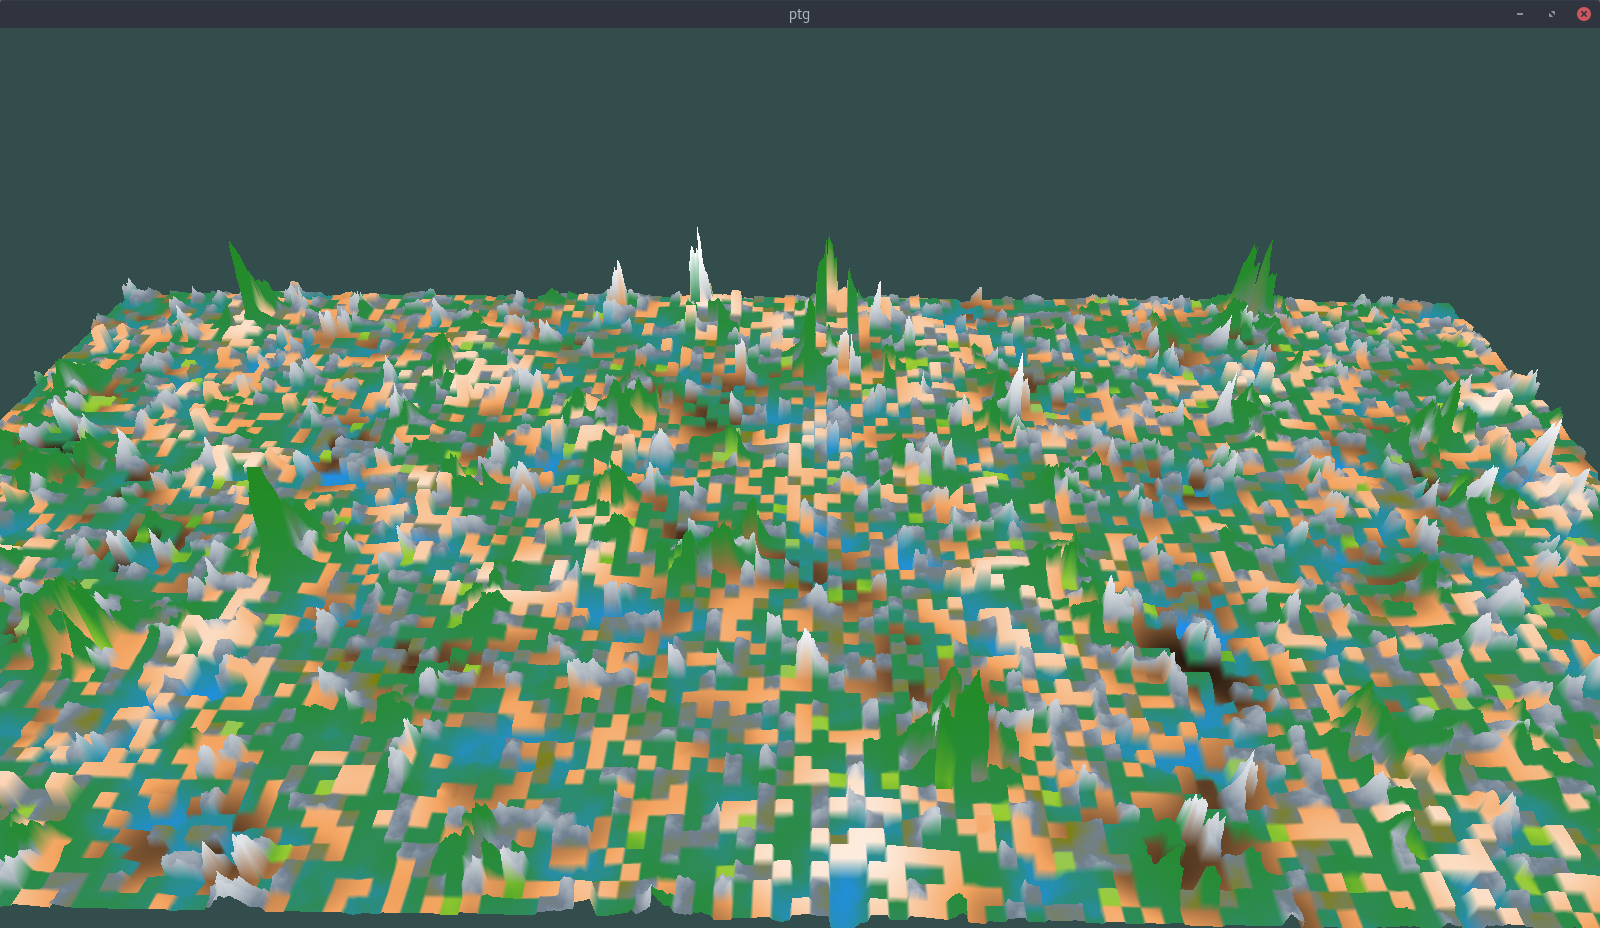
\includegraphics[width=0.31\textwidth]{figuras/re2bfb/fb/05b32.png}\label{fig:re2bfb_fb_05b32}}\hspace{0.1cm}
     \subfloat[][$fb = 1$]{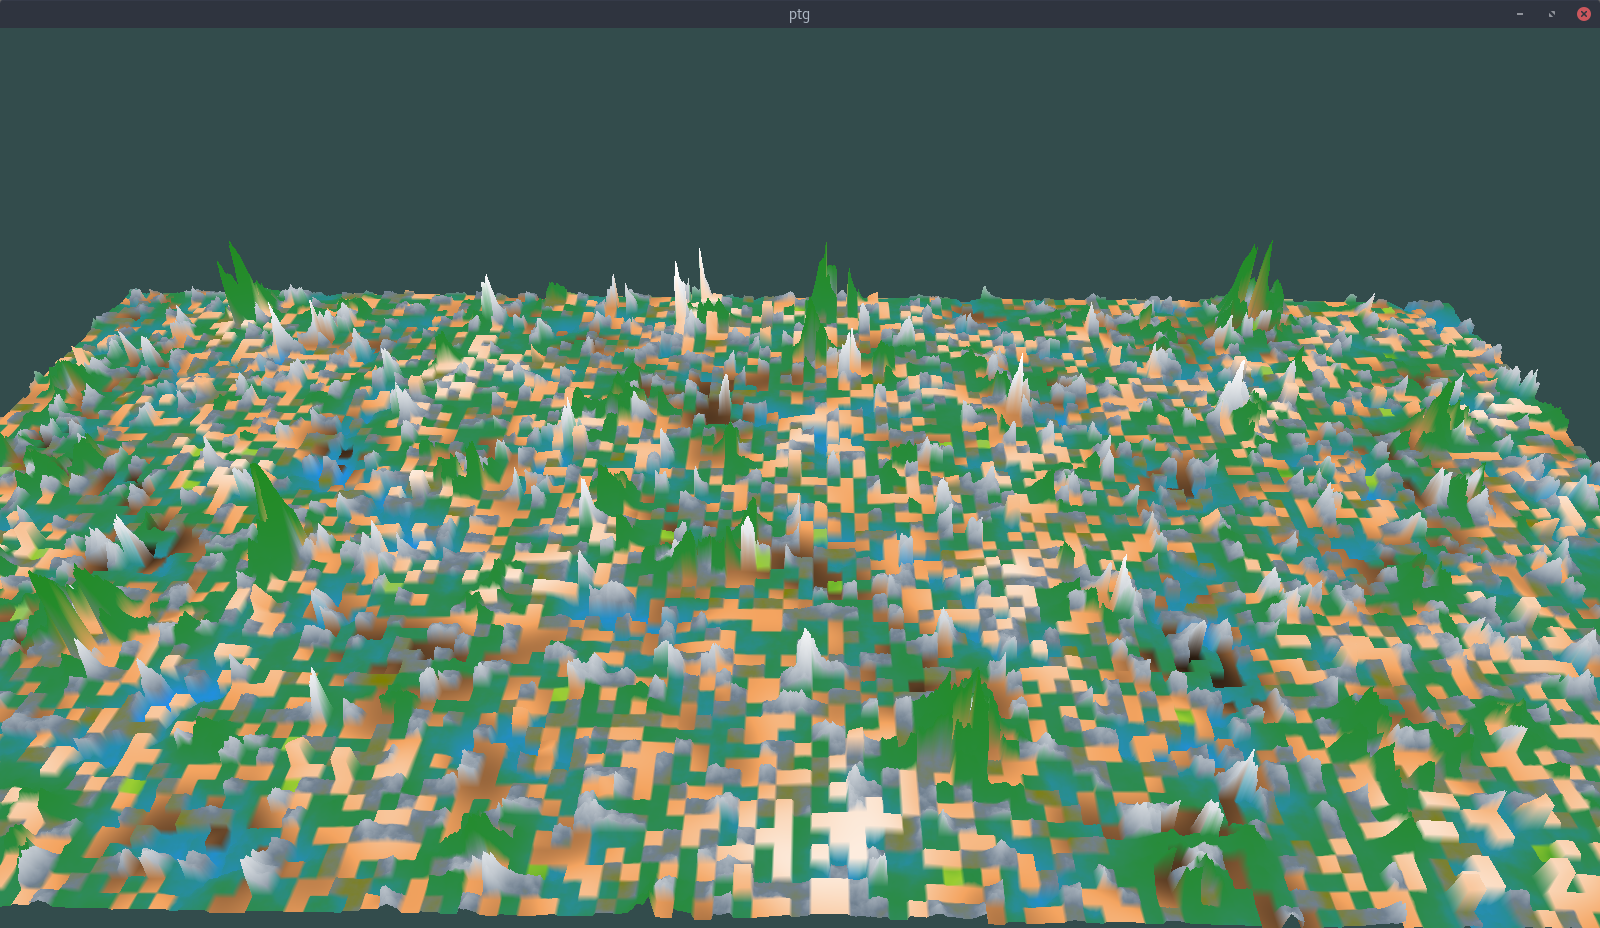
\includegraphics[width=0.31\textwidth]{figuras/re2bfb/fb/1b32.png}\label{fig:re2bfb_fb_1b32}}\hspace{0.1cm}
     \subfloat[][$fb = 8$]{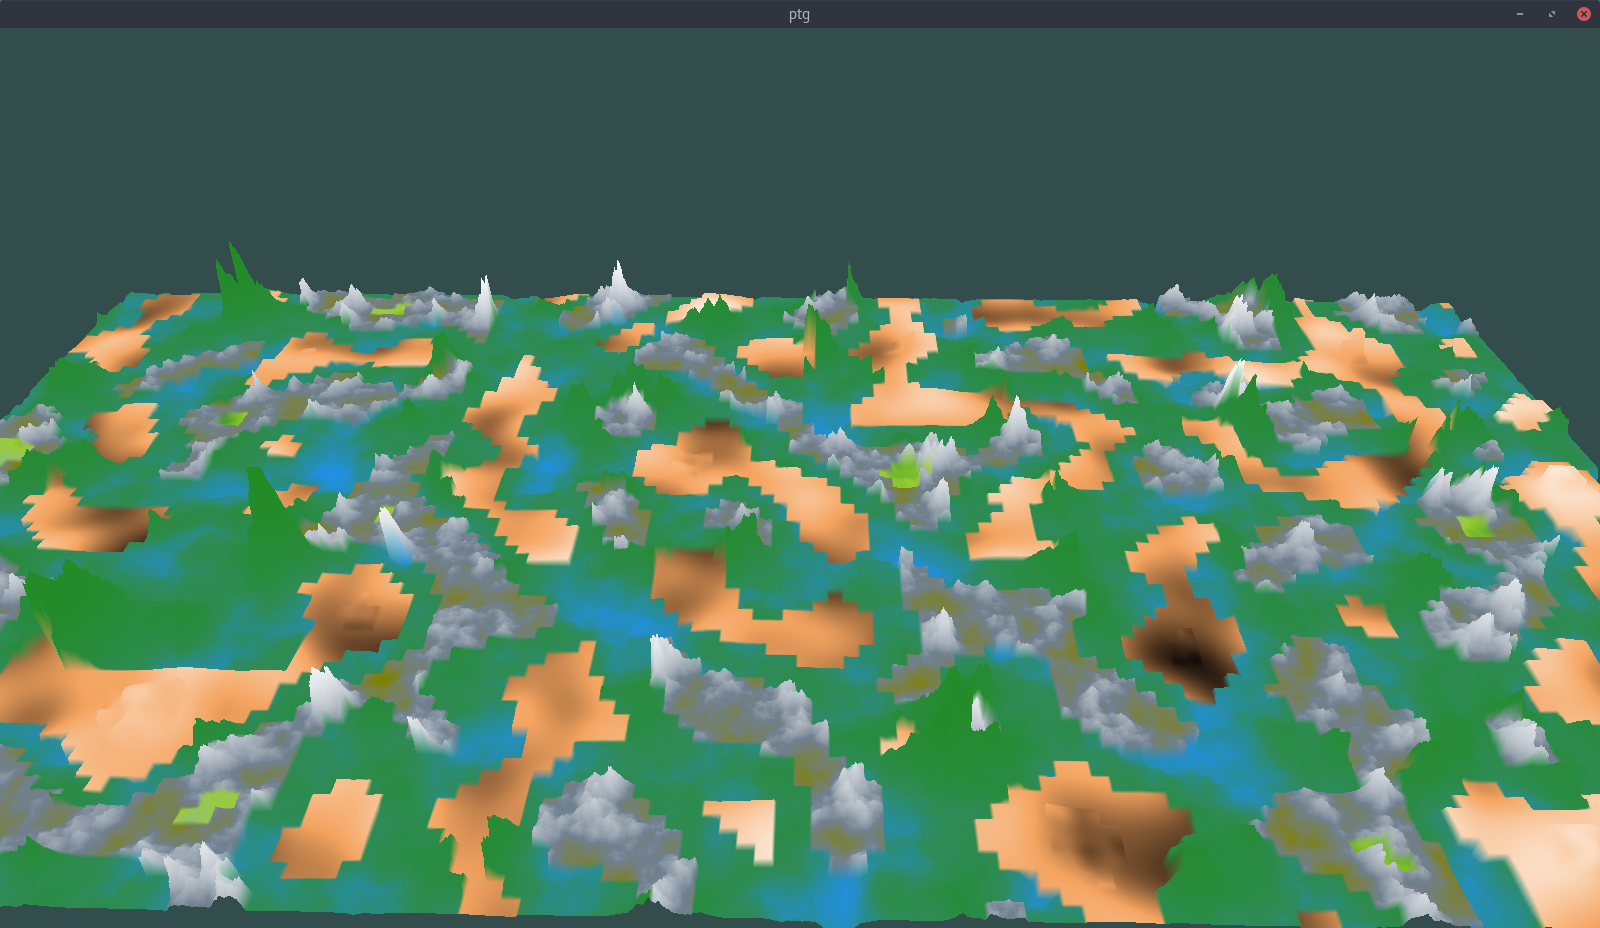
\includegraphics[width=0.31\textwidth]{figuras/re2bfb/fb/8b32.png}\label{fig:re2bfb_fb_8b32}}\\
     \subfloat[][$fb = 16$]{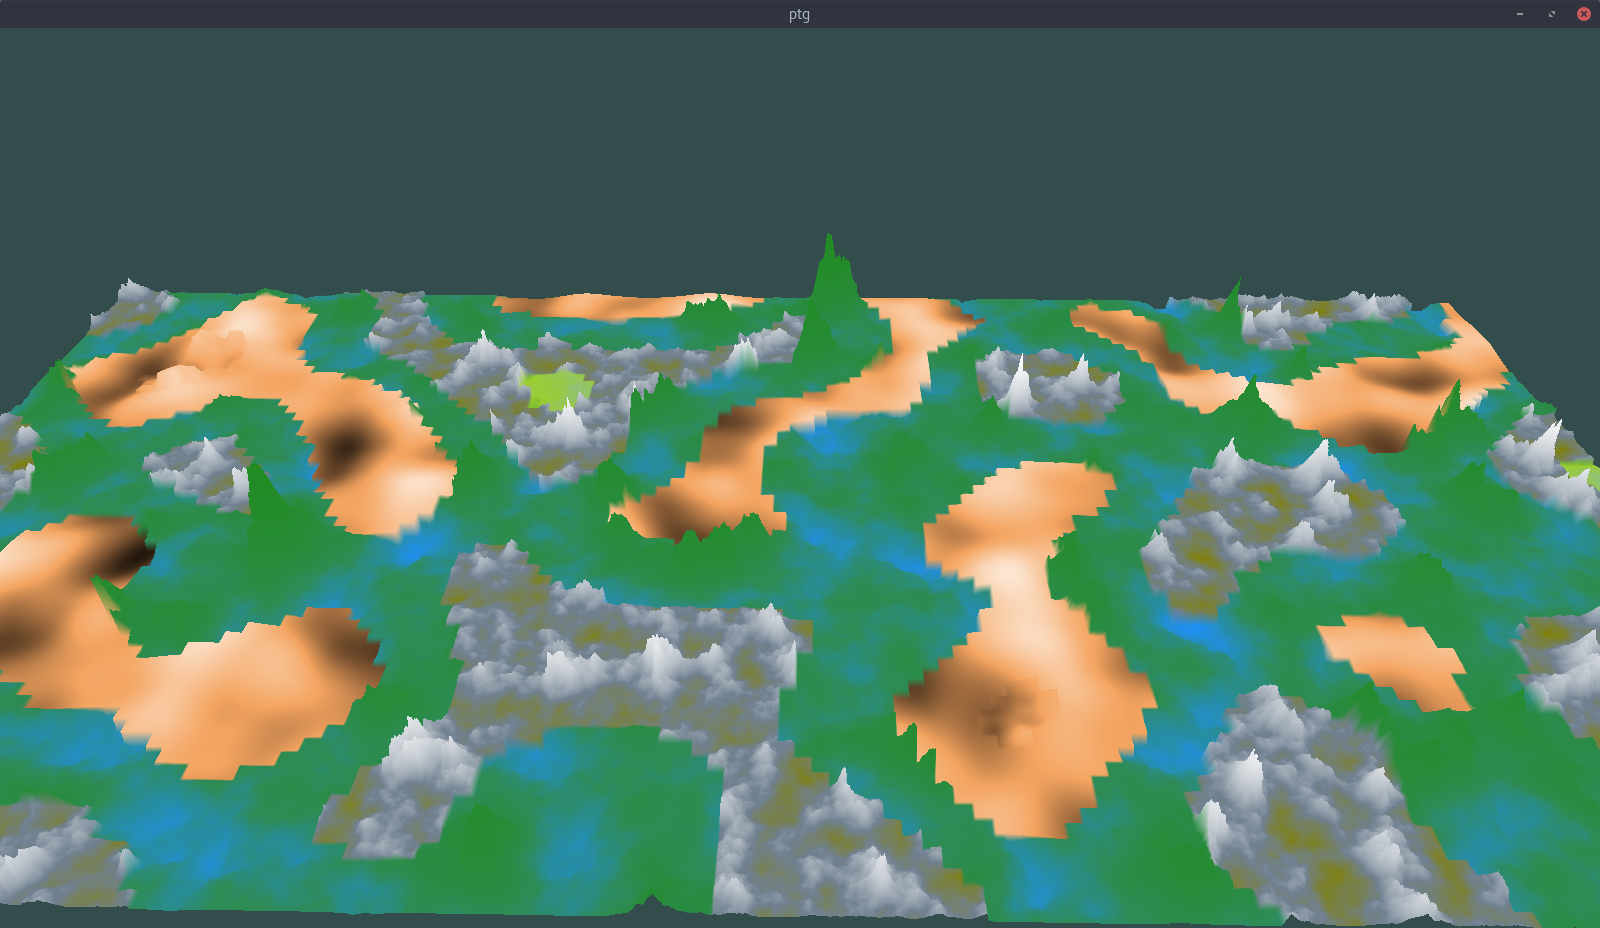
\includegraphics[width=0.31\textwidth]{figuras/re2bfb/fb/16b32.png}\label{fig:re2bfb_fb_16b32}}\hspace{0.1cm}
     \subfloat[][$fb = 32$]{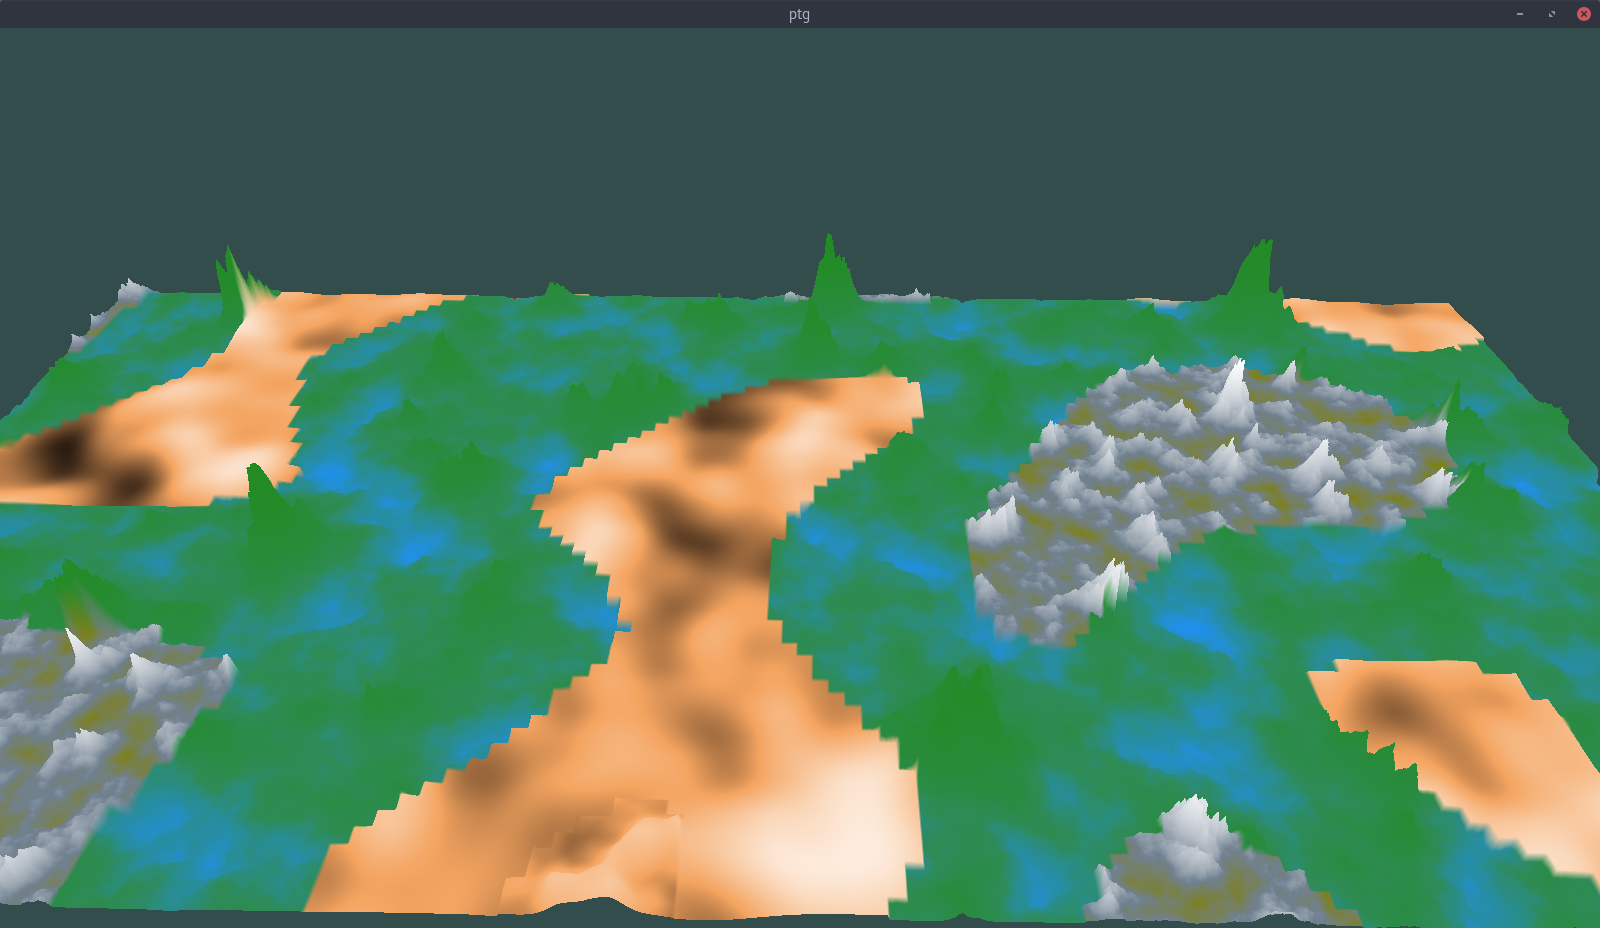
\includegraphics[width=0.31\textwidth]{figuras/re2bfb/fb/32b32.png}\label{fig:re2bfb_fb_32b32}}\hspace{0.1cm}
     \subfloat[][$fb = 64$]{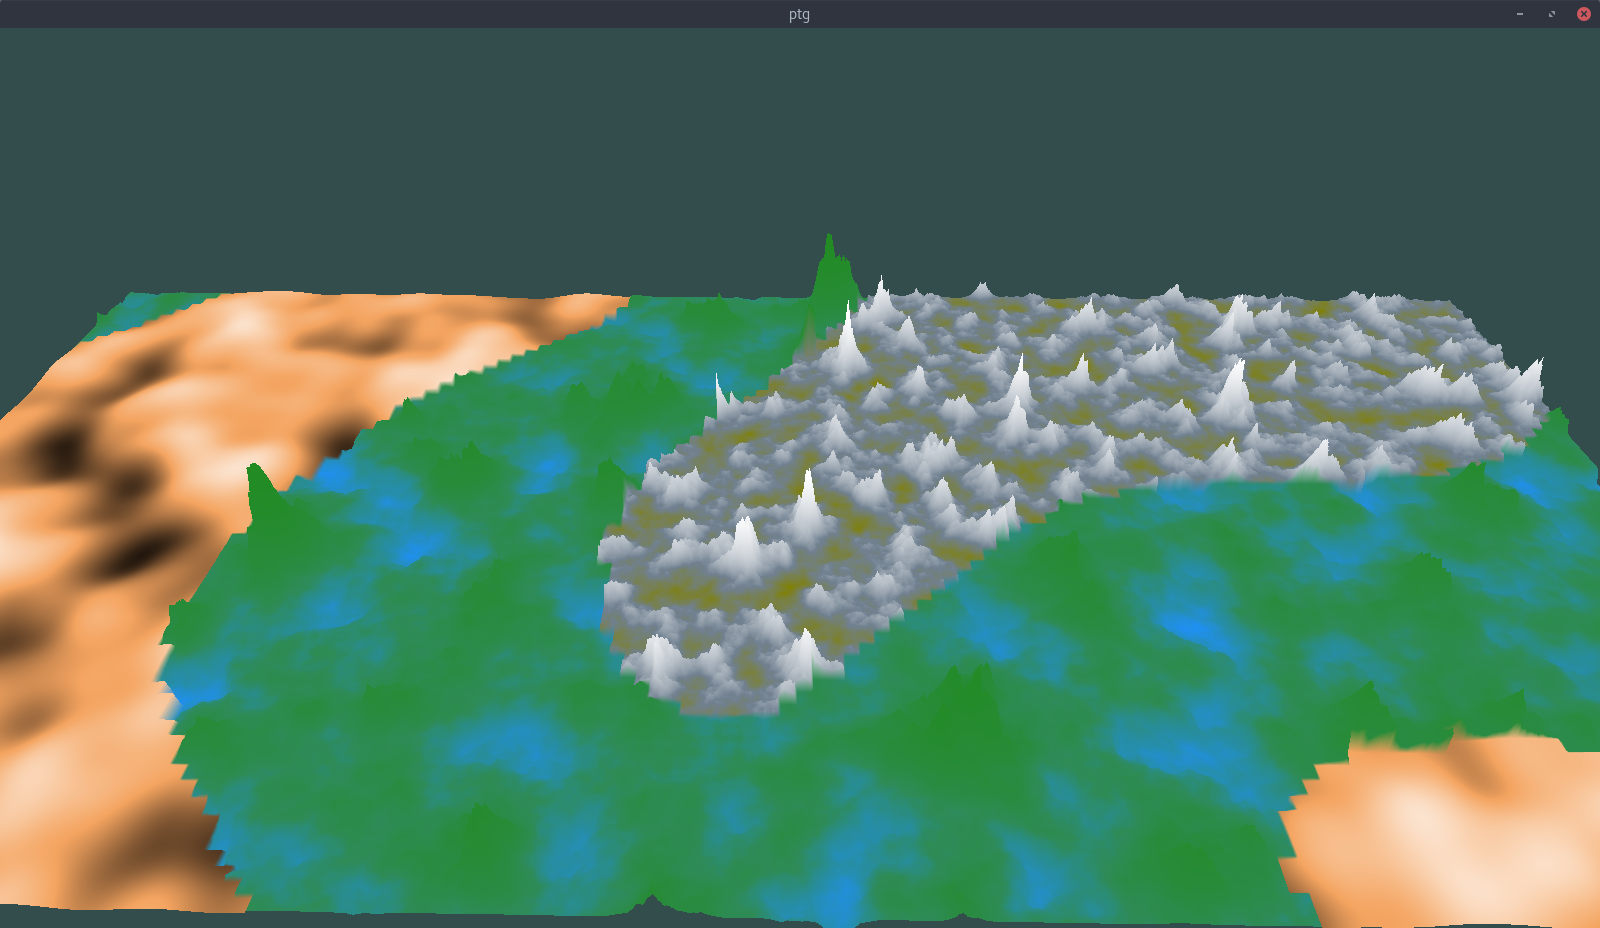
\includegraphics[width=0.31\textwidth]{figuras/re2bfb/fb/64b32.png}\label{fig:re2bfb_fb_64b32}}
     
     \caption{Diferentes frequências de biomas, para tamanho de área $b = 32$.}
     
     \label{fig:comparandofreqdebiomasyeah}
     % usar \hspace{0.1cm}, é gambiarra mas funciona
\end{figure}

Para a fronteira entre os biomas distintos obter uma forma mais orgânica, e deixar o 
terreno com melhor jogabilidade, já que descontinuidade no terreno seria um empecilho em alguns jogos.
Foi feito interpolação linear nas ocorrências de fronteiras, nas diagonais de área de bioma foi 
usado interpolação bilinear, já que este cobre o pior caso, que seria fronteira entre quatro biomas distintos,
mostrado nas figuras \ref{fig:wcborder4biomes}.%debug: figura pior caso ref aqui

A distância em que uma interpolação começa a ser feita é definida pelo parâmetro $l$,
quanto maior for $l$ maior será a área de interpolação e mais suave será transição de um bioma para o outro,
sua influência pode ser comparada nas imagens \ref{fig:borderslcomp}.

\begin{figure}[H]
     \centering
     \subfloat[][Sem interpolação]{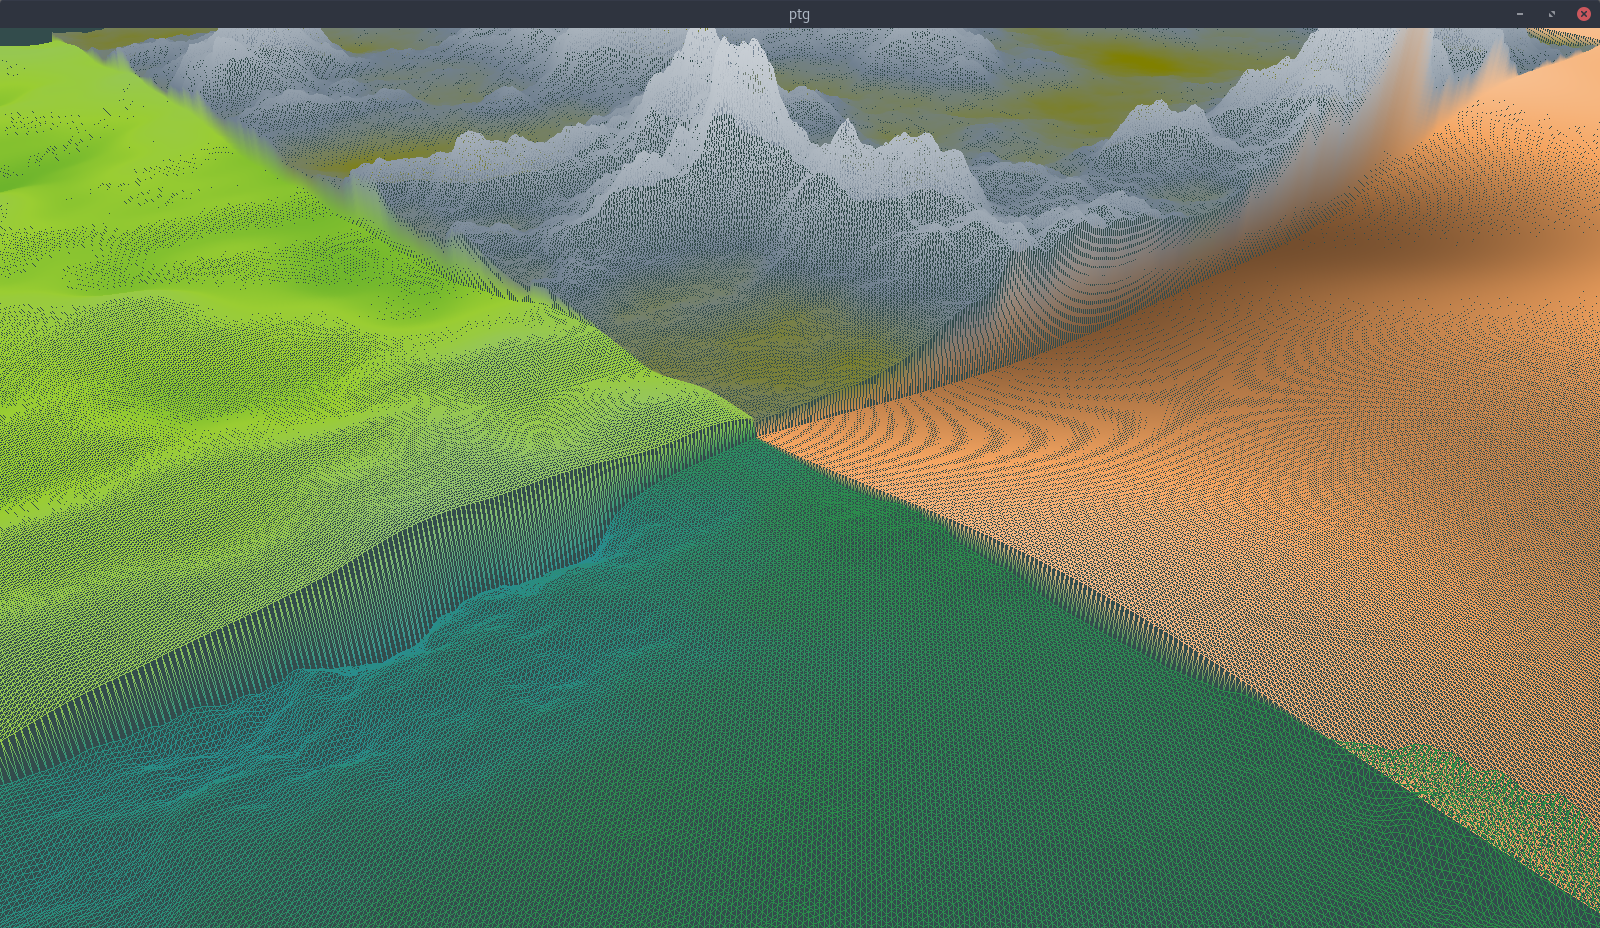
\includegraphics[width=0.48\textwidth]{figuras/wc/wcmni.png}\label{fig:wc_wcmni}}\hspace{0.1cm}
     \subfloat[][Com interpolação]{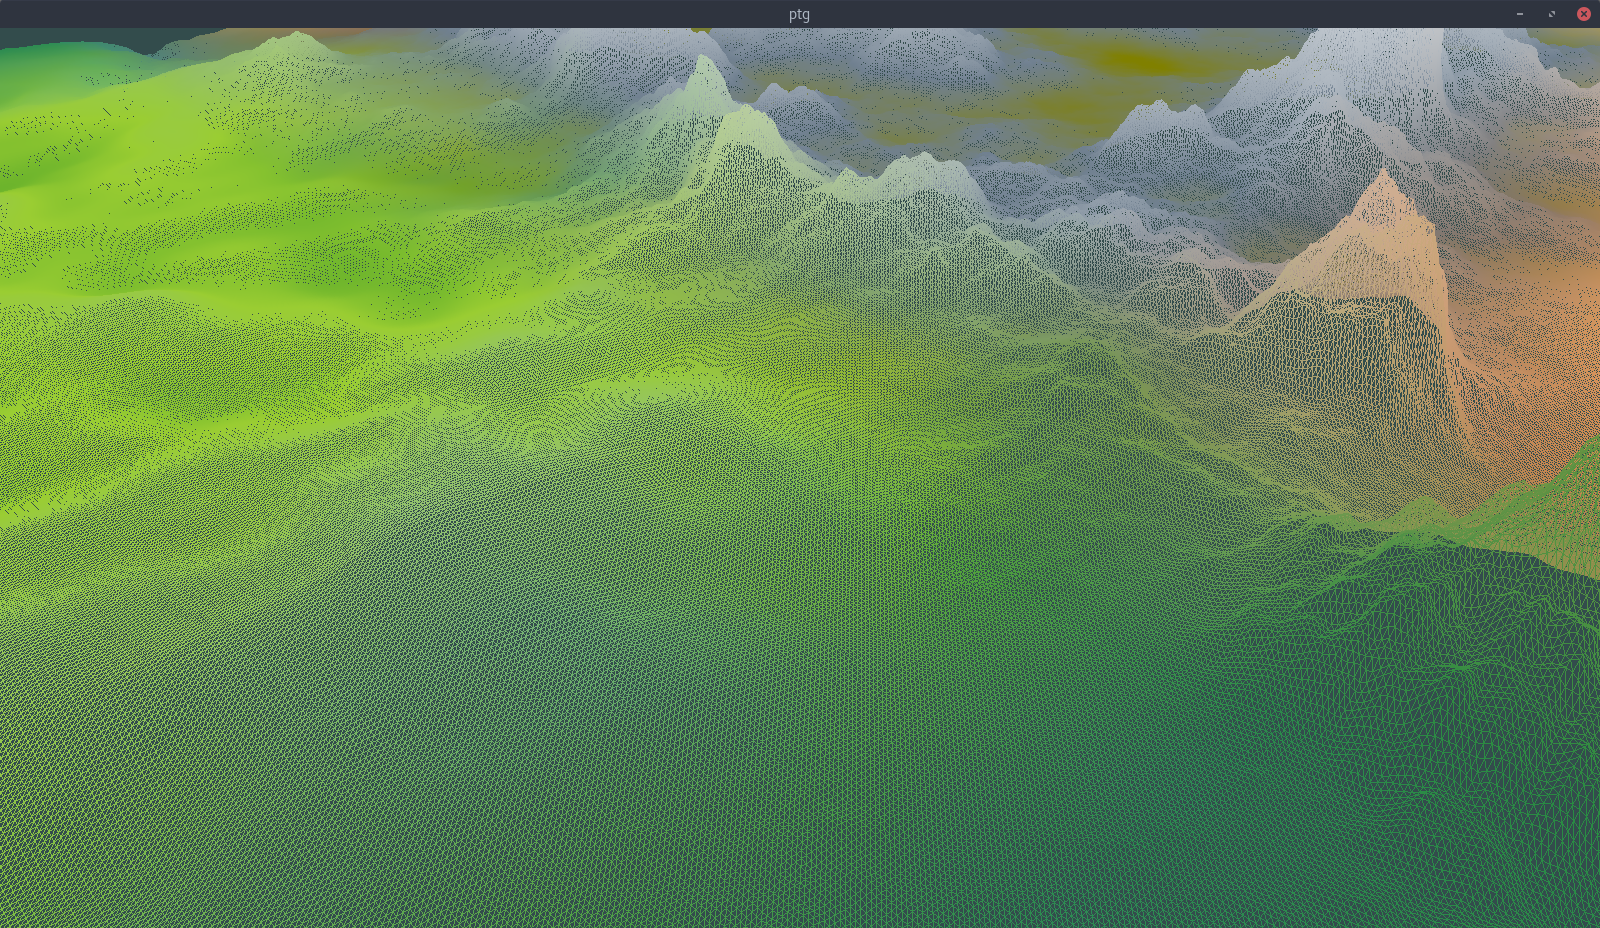
\includegraphics[width=0.48\textwidth]{figuras/wc/wcmi.png}\label{fig:wc_wcmi}}
     
     \caption{Fronteira entre quatro biomas.}
     
     \label{fig:wcborder4biomes}
     % usar \hspace{0.1cm}, é gambiarra mas funciona
\end{figure}

\begin{figure}[H]
     \centering
     \subfloat[][Sem interpolação]{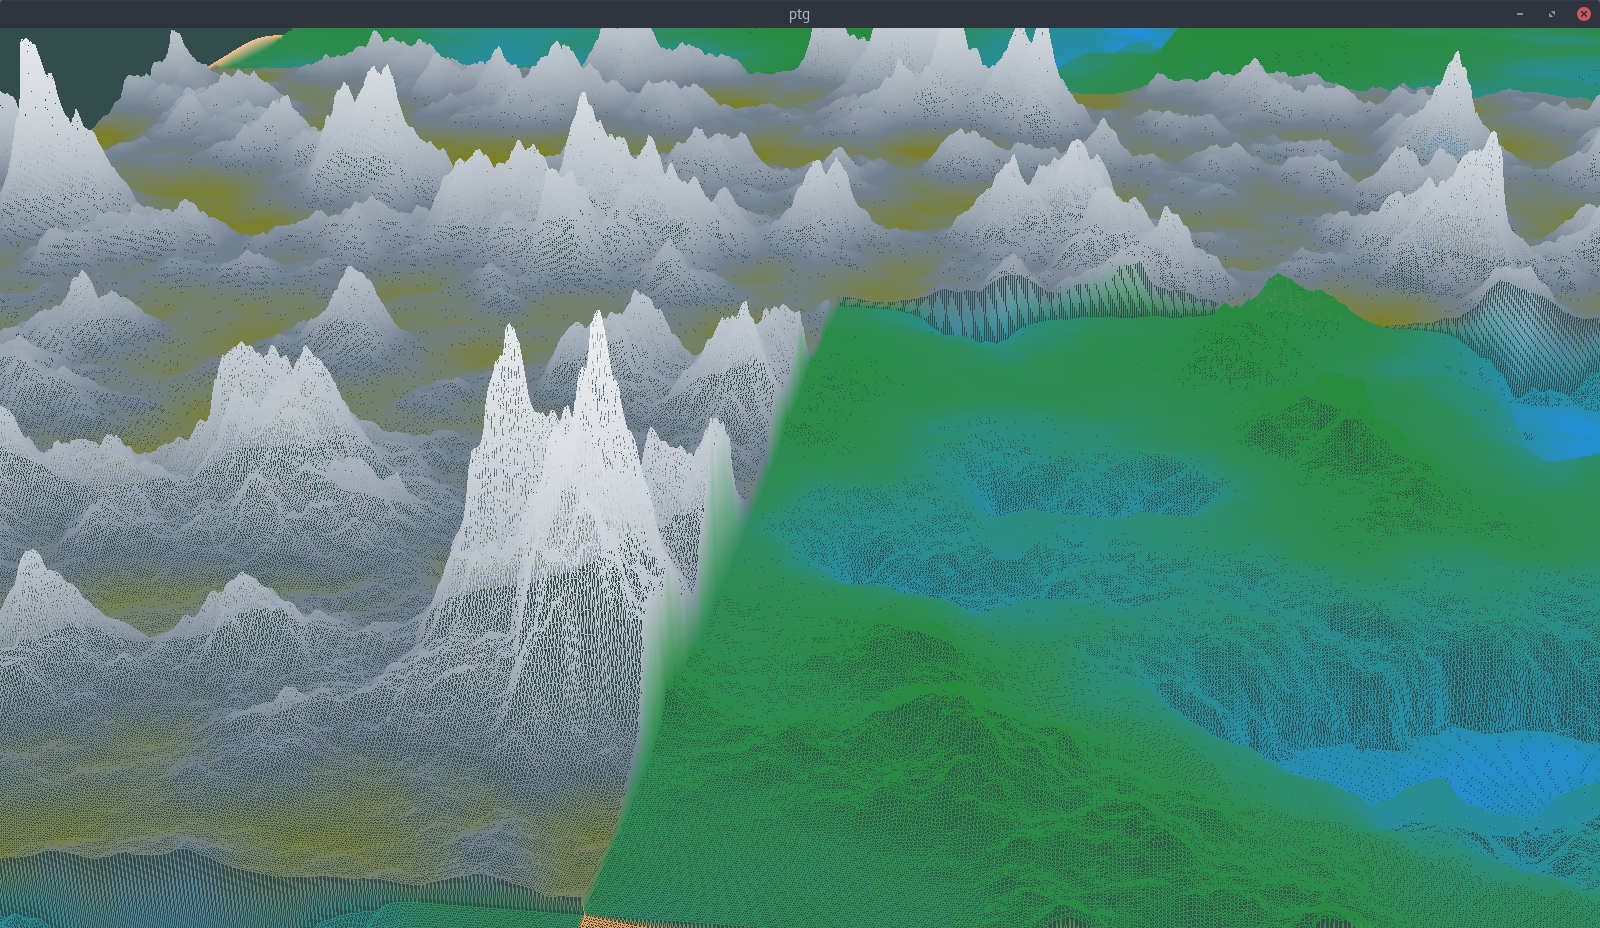
\includegraphics[width=0.48\textwidth]{figuras/borders/0lm.png}\label{fig:borders_0lm}}\hspace{0.1cm}
     \subfloat[][$l = 8$]{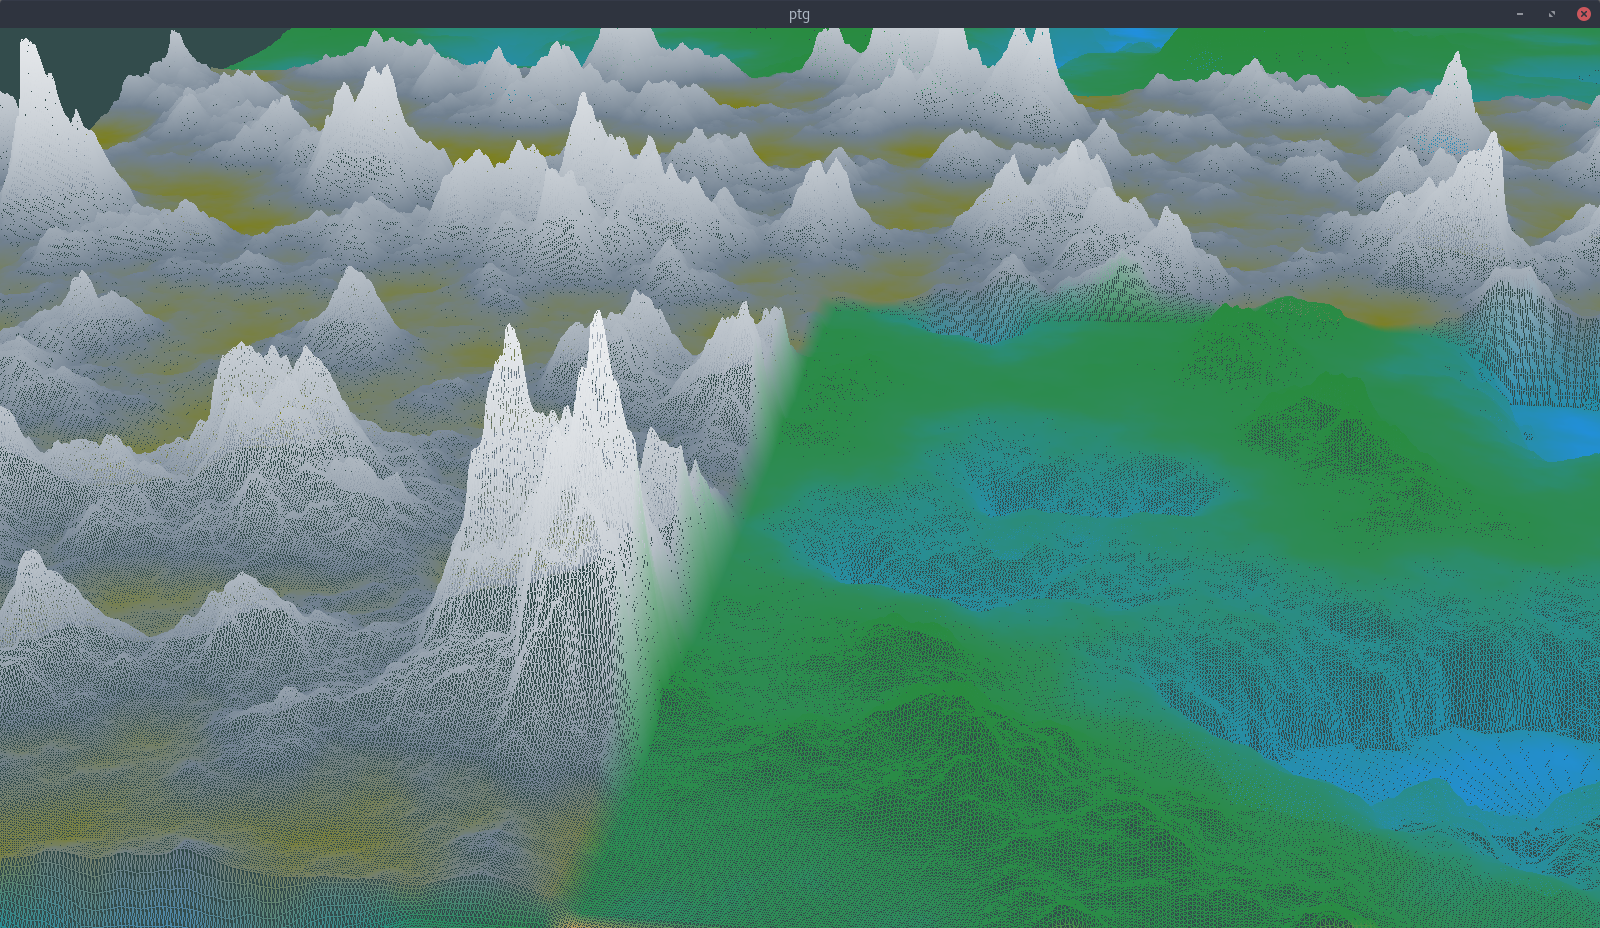
\includegraphics[width=0.48\textwidth]{figuras/borders/8lm.png}\label{fig:borders_8lm}}\\
     \subfloat[][$l = 128$]{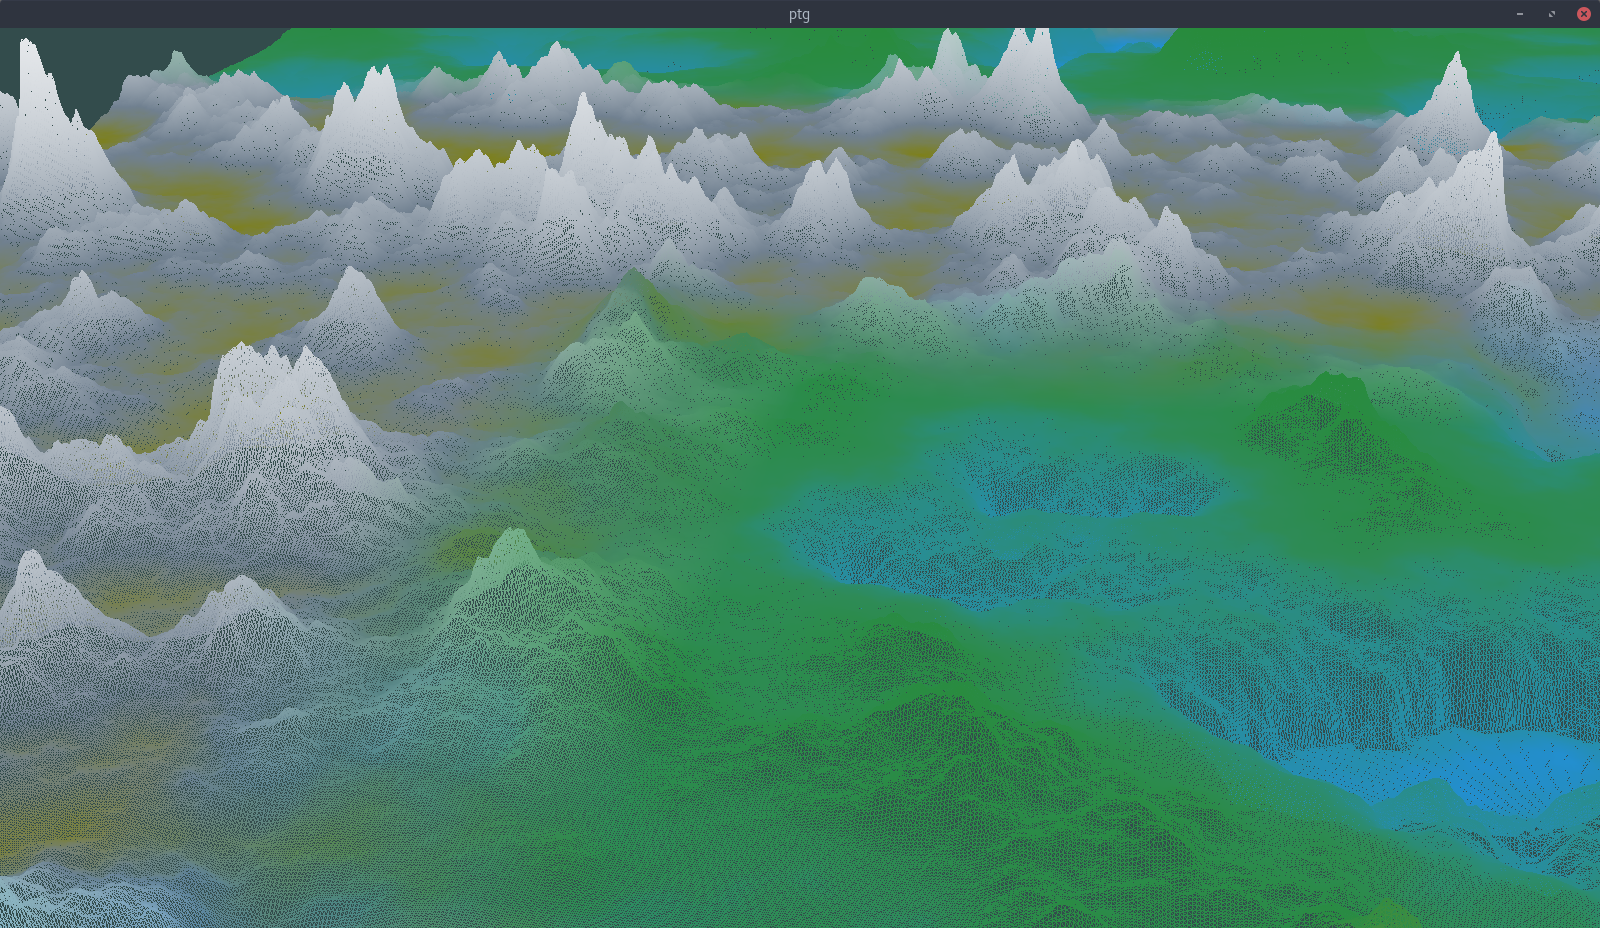
\includegraphics[width=0.48\textwidth]{figuras/borders/128lm.png}\label{fig:borders_128lm}}\hspace{0.1cm}
     \subfloat[][$l = 255$]{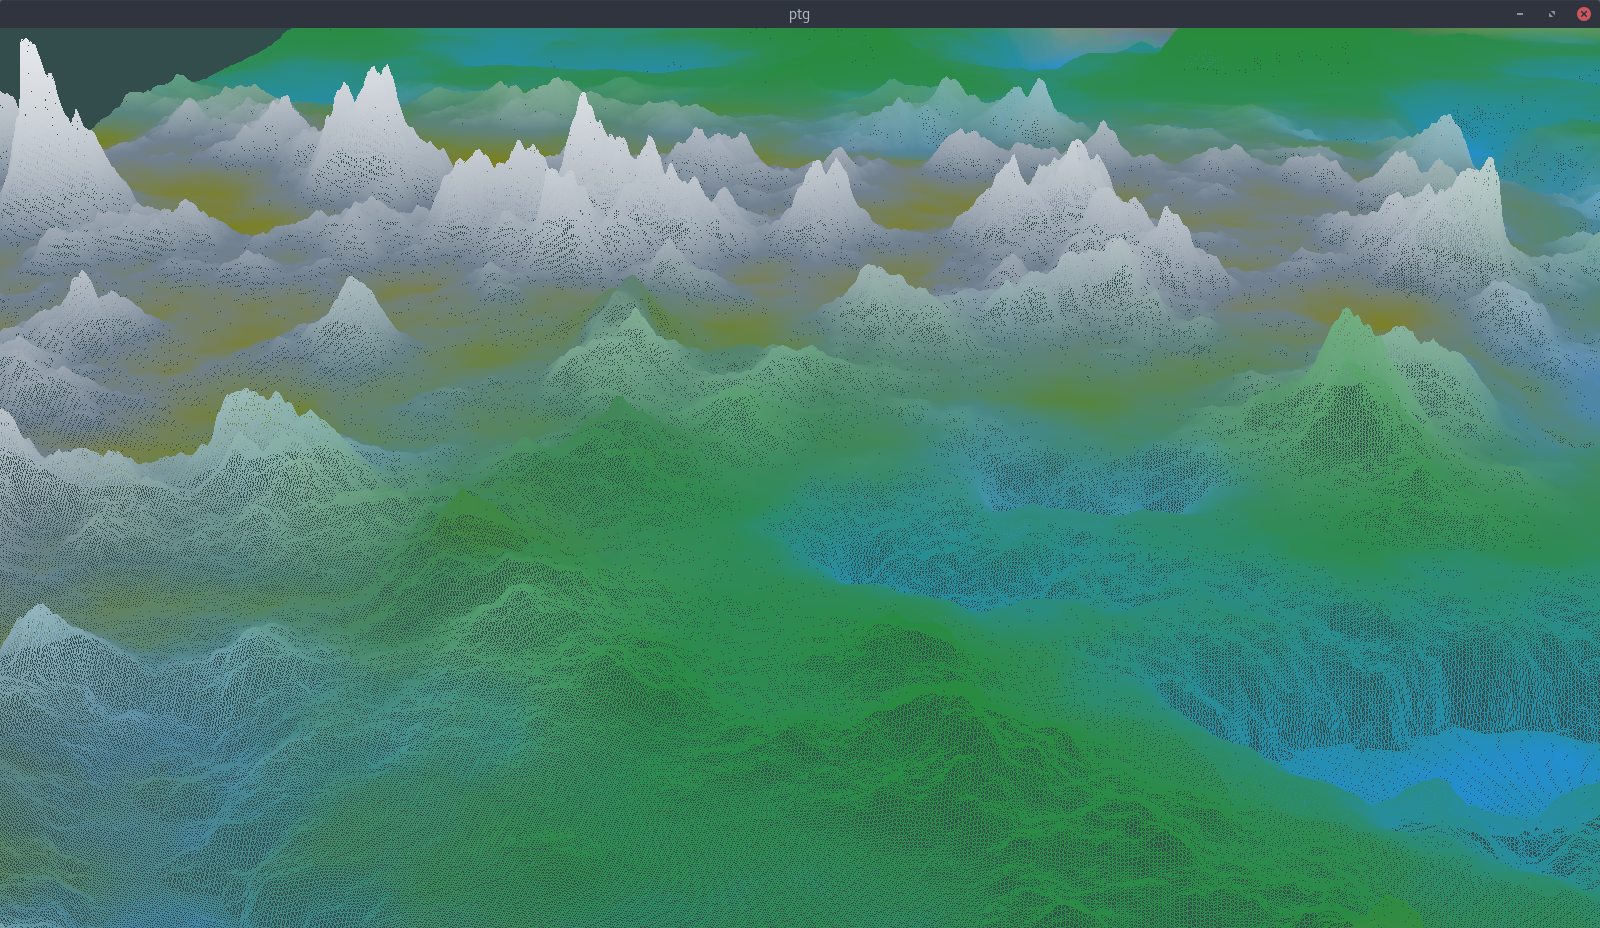
\includegraphics[width=0.48\textwidth]{figuras/borders/255lm.png}\label{fig:borders_255lm}}
     
     
     \caption{Comparando $l$ nas fronteiras.}
     
     \label{fig:borderslcomp}
     % usar \hspace{0.1cm}, é gambiarra mas funciona
\end{figure}






%\begin{figure}[H]
%    \centering
%    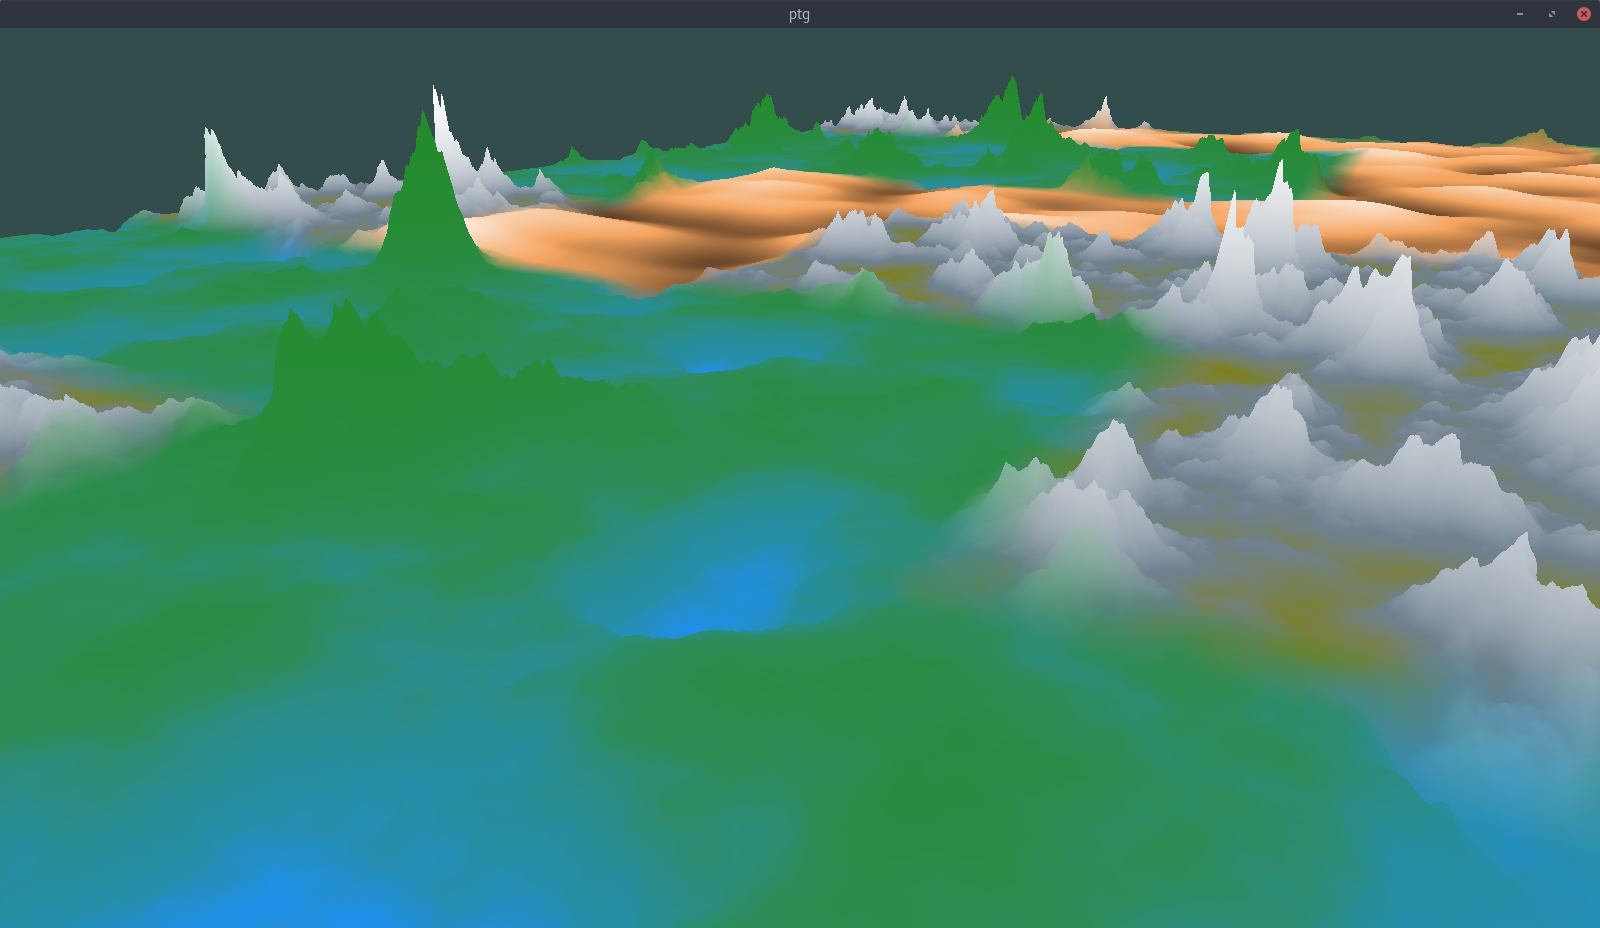
\includegraphics[width=0.5\textwidth]{figuras/ssFinalResult.png}
%    \caption{Resultado final}
%    \label{fig:ssFinalResult}
%\end{figure}
%
%\begin{figure}[H]
%     \centering
%     \subfloat[][$b = 260$]{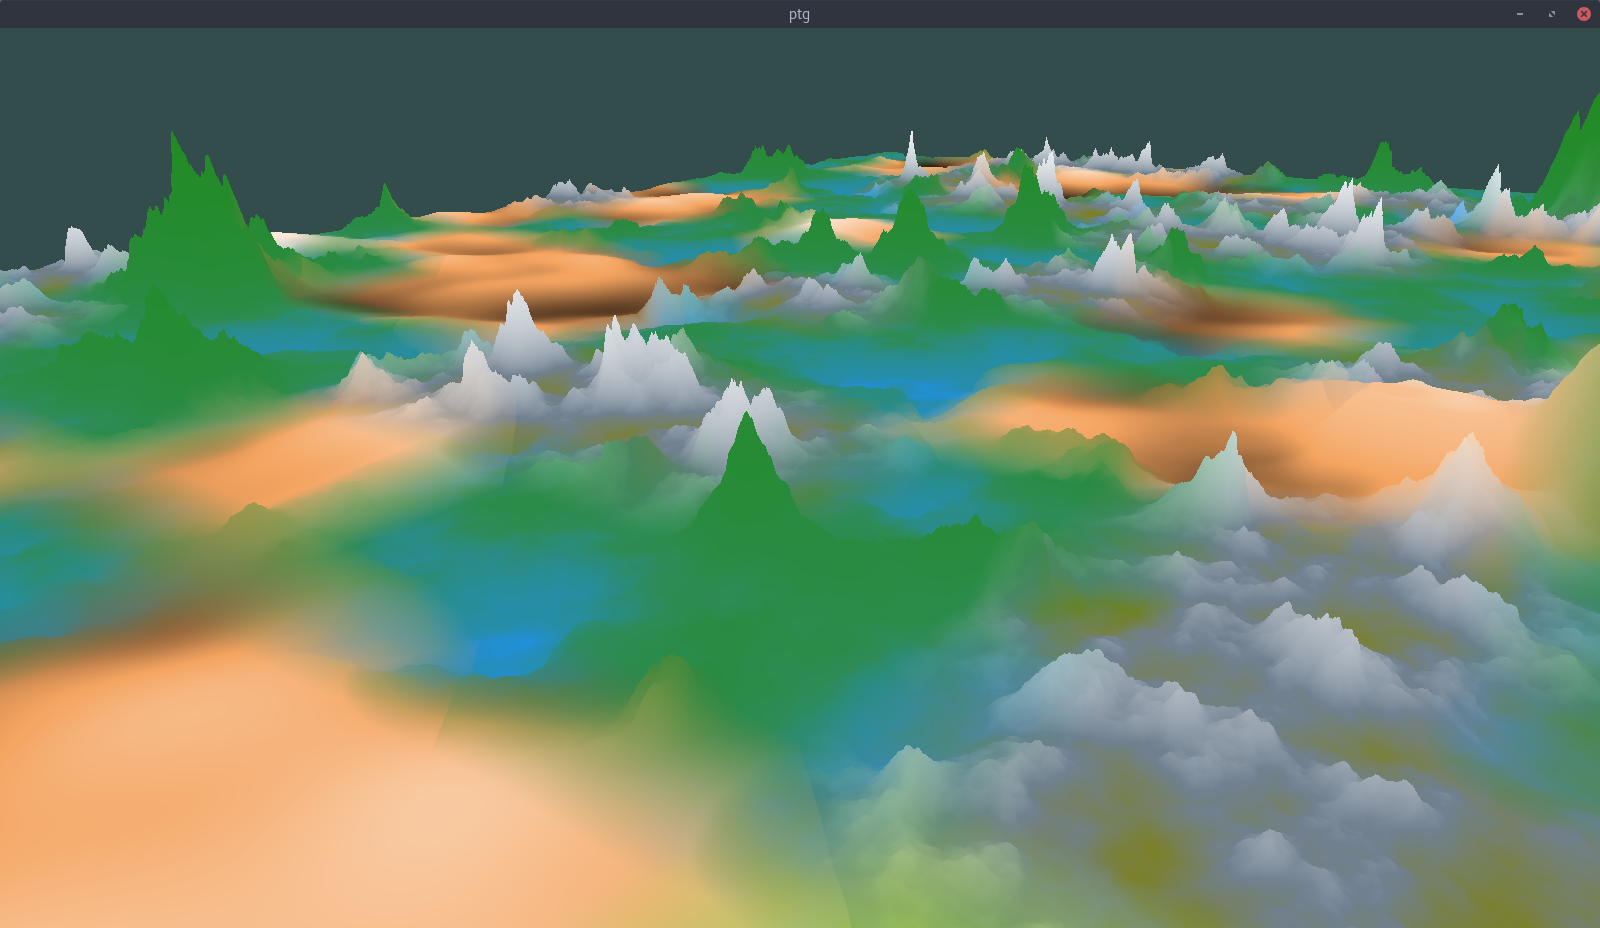
\includegraphics[width=0.48\textwidth]{figuras/resultados/b/resultSeed3Deltav05k2048b260l128.png}\label{fig:b260}}\hspace{0.1cm}
%     \subfloat[][$b = 512$]{\includegraphics[width=0.48\textwidth]{figuras/resultados/b/resultSeed3Deltav05k2048b512l128.png}\label{fig:b512}}\\
%     \subfloat[][$b = 1024$]{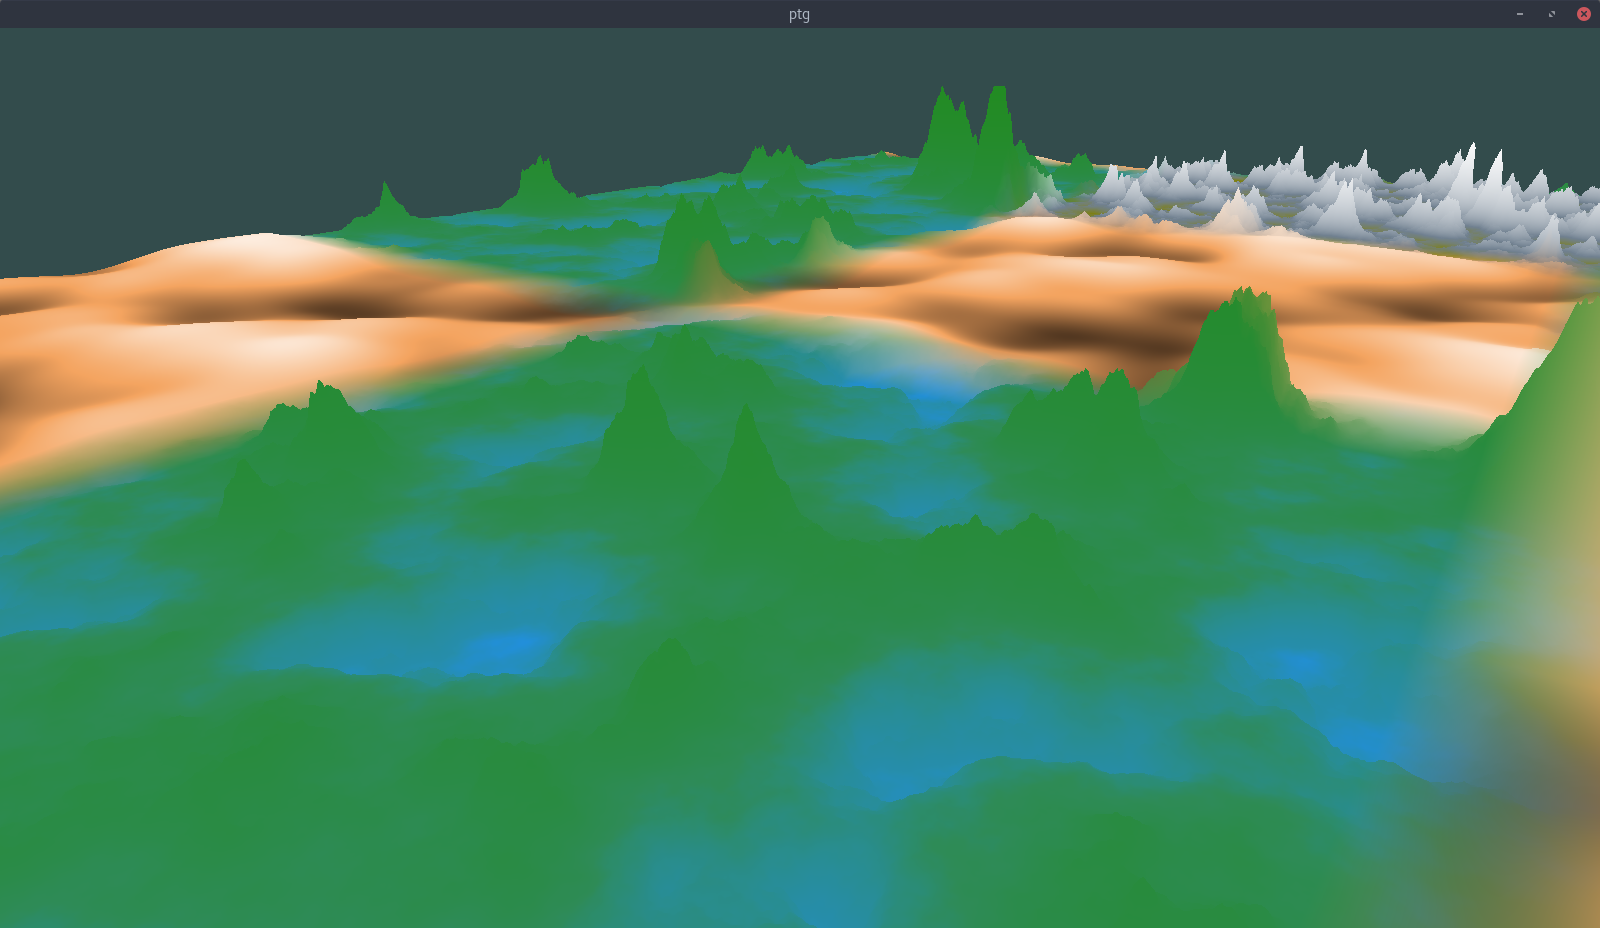
\includegraphics[width=0.48\textwidth]{figuras/resultados/b/resultSeed3Deltav05k2048b1024l128.png}\label{fig:b1024}}\hspace{0.1cm}
%     \subfloat[][$b = 1500$]{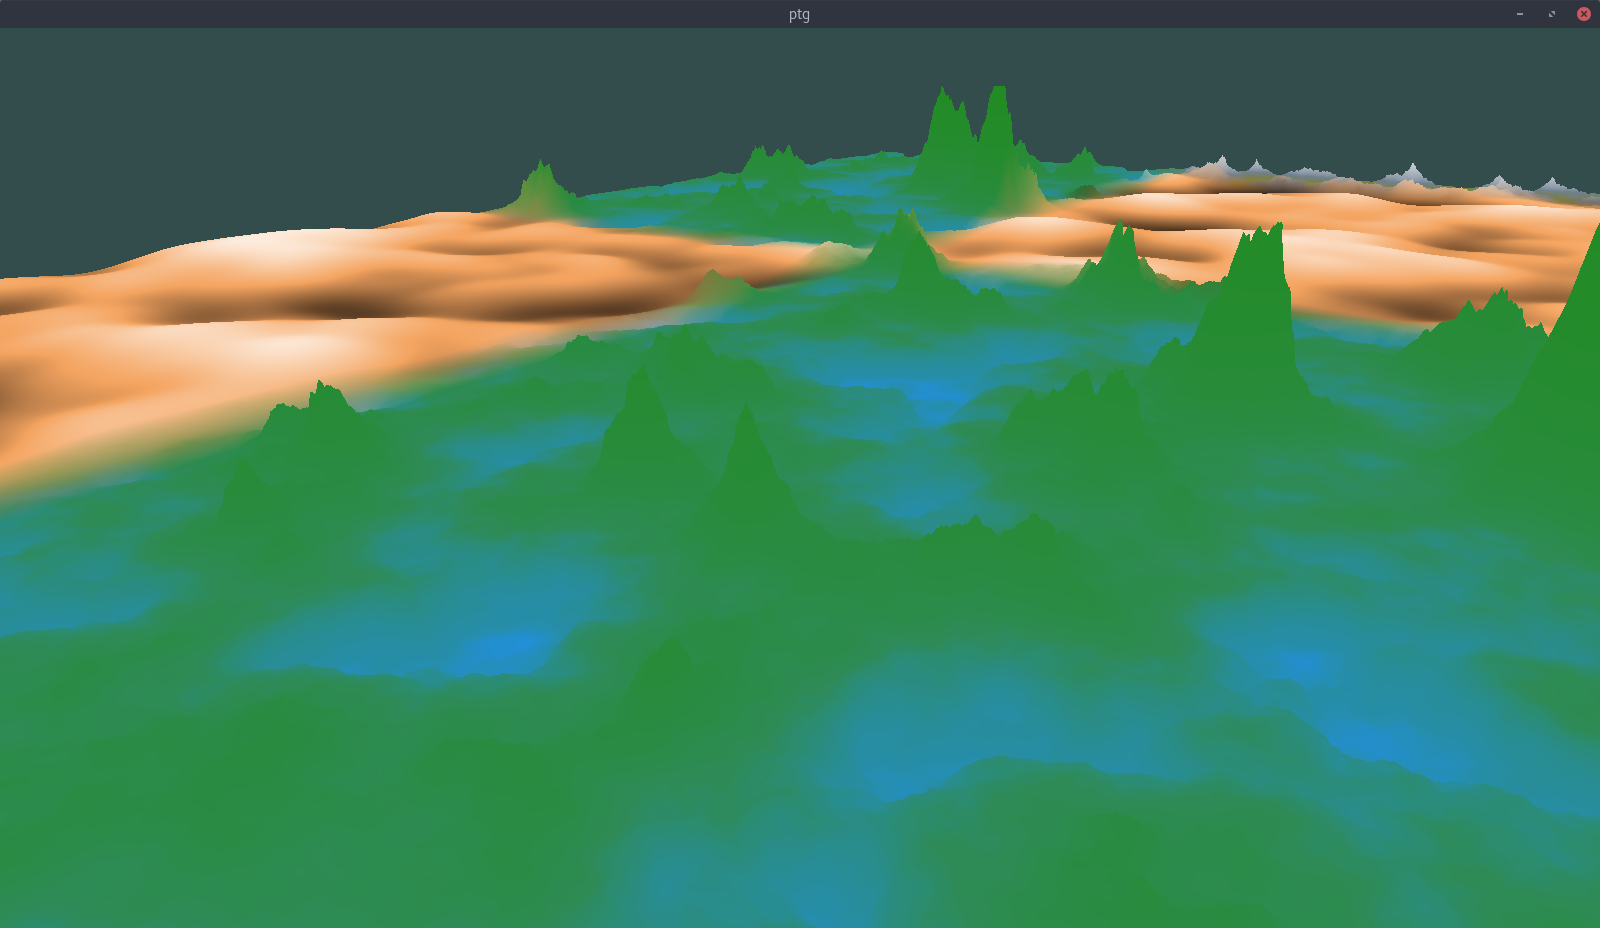
\includegraphics[width=0.48\textwidth]{figuras/resultados/b/resultSeed3Deltav05k2048b1500l128.png}\label{fig:b1500}}
%     
%     \caption{Tamanho de cada Bioma.}
%     
%     \label{fig:biomeComp}
%     % usar \hspace{0.1cm}, é gambiarra mas funciona
%\end{figure}
%
%\begin{figure}[H]
%     \centering
%     \subfloat[][$l = 2$]{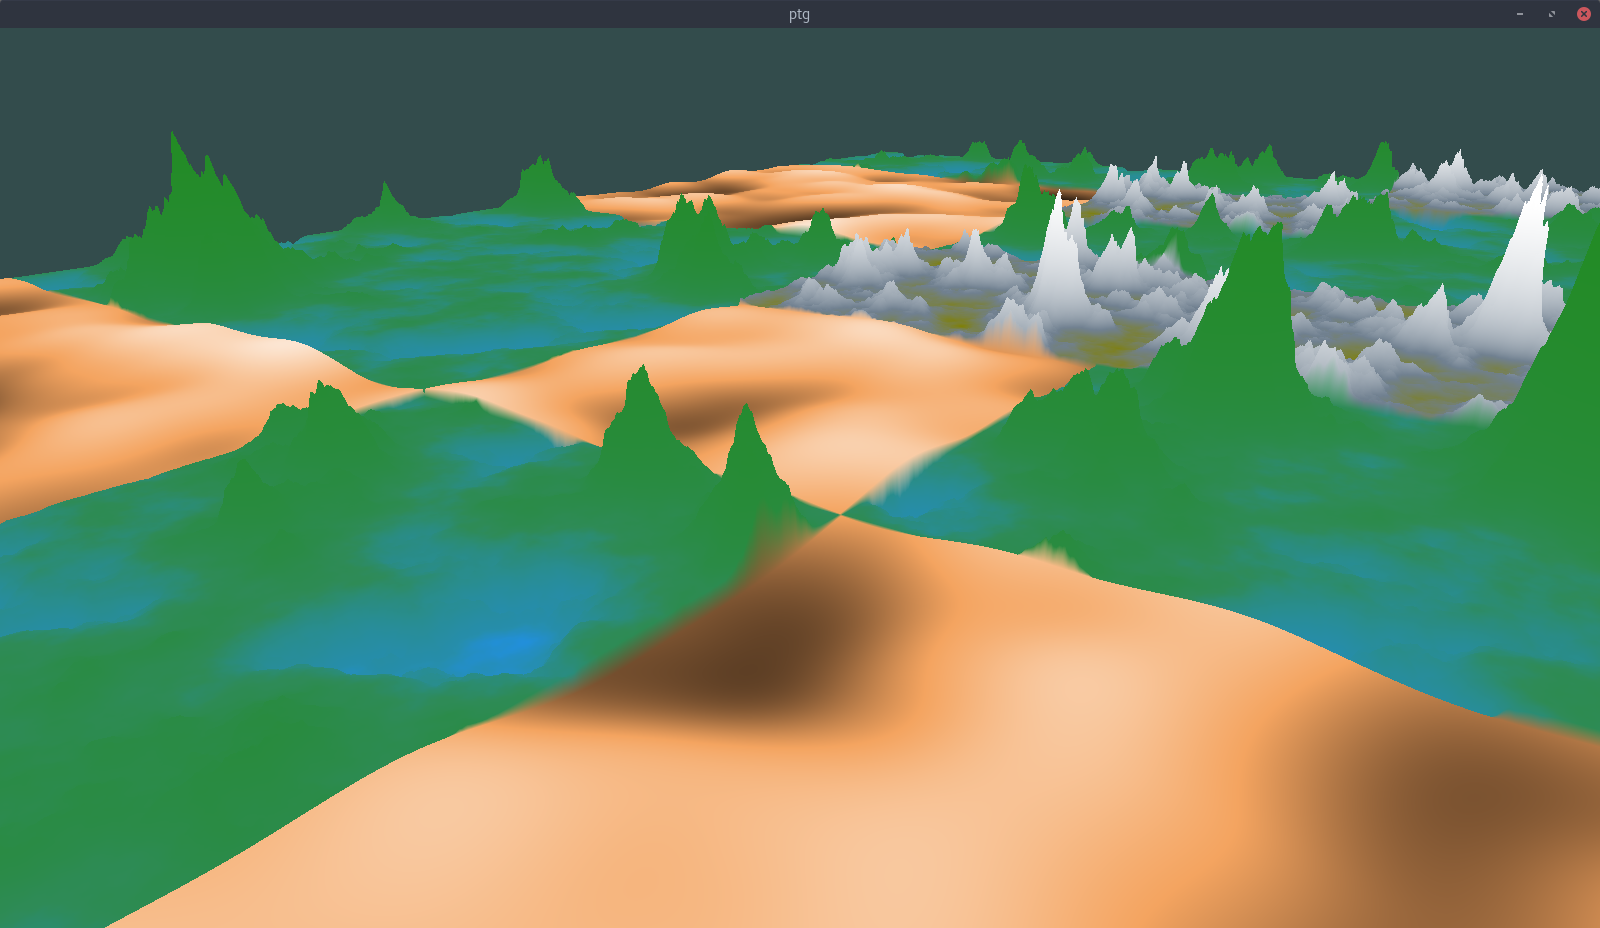
\includegraphics[width=0.48\textwidth]{figuras/resultados/l/resultSeed3Deltav05k2048b512l2.png}\label{fig:l2}}\hspace{0.1cm}
%     \subfloat[][$l = 64$]{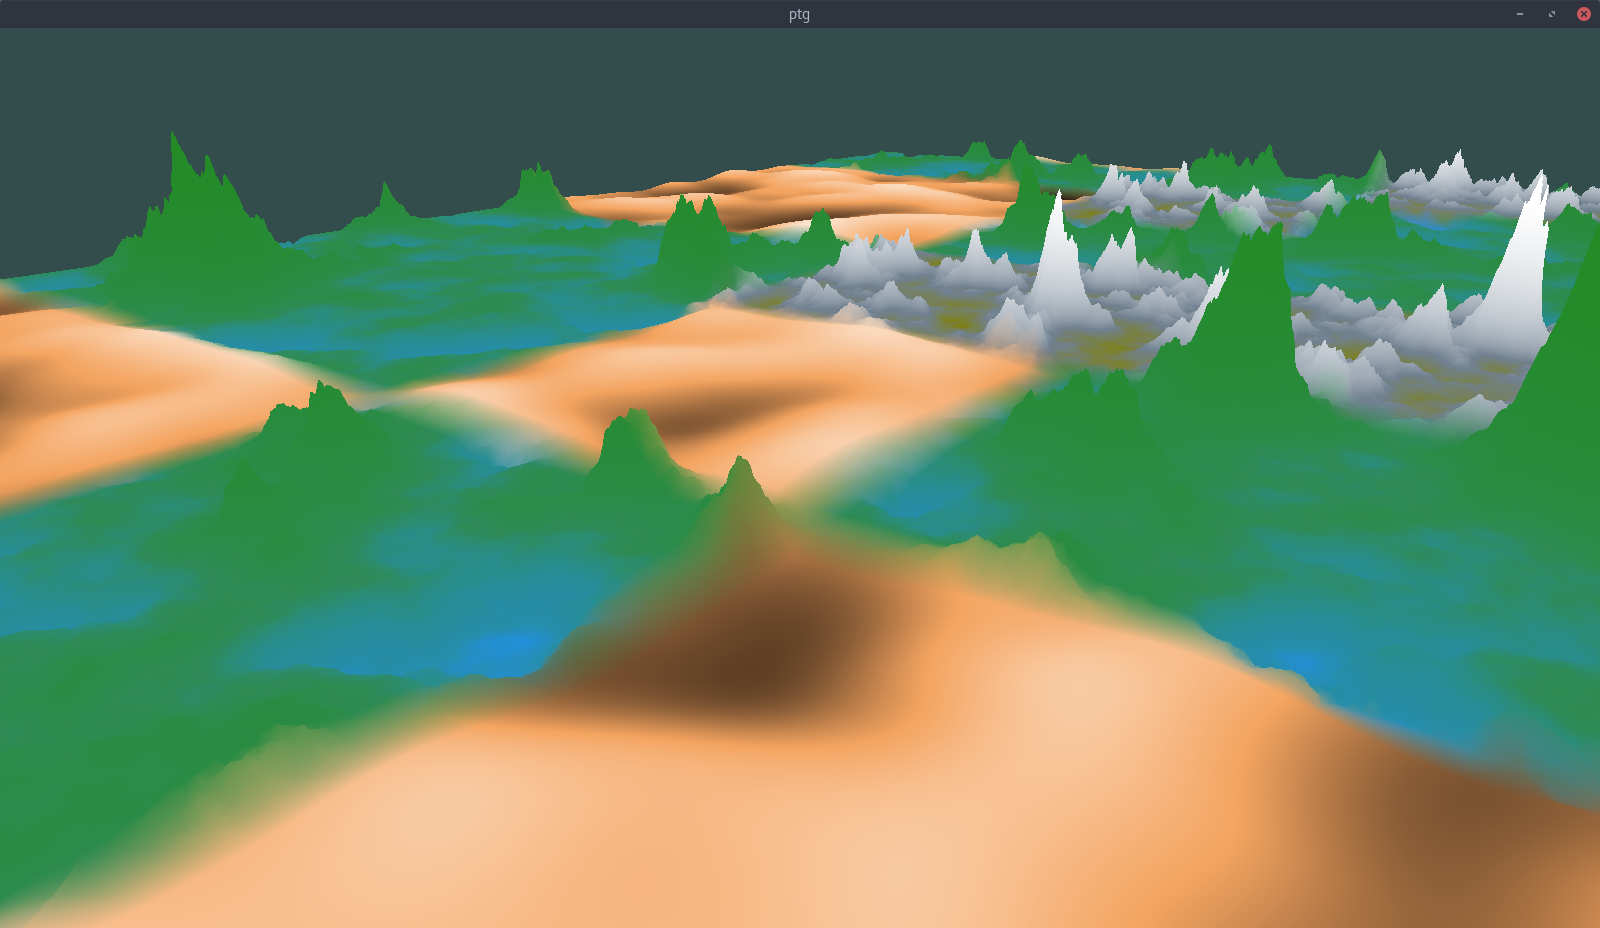
\includegraphics[width=0.48\textwidth]{figuras/resultados/l/resultSeed3Deltav05k2048b512l64.png}\label{fig:l64}}\\
%     \subfloat[][$l = 128$]{\includegraphics[width=0.48\textwidth]{figuras/resultados/l/resultSeed3Deltav05k2048b512l128.png}\label{fig:l128}}\hspace{0.1cm}
%     \subfloat[][$l = 256$]{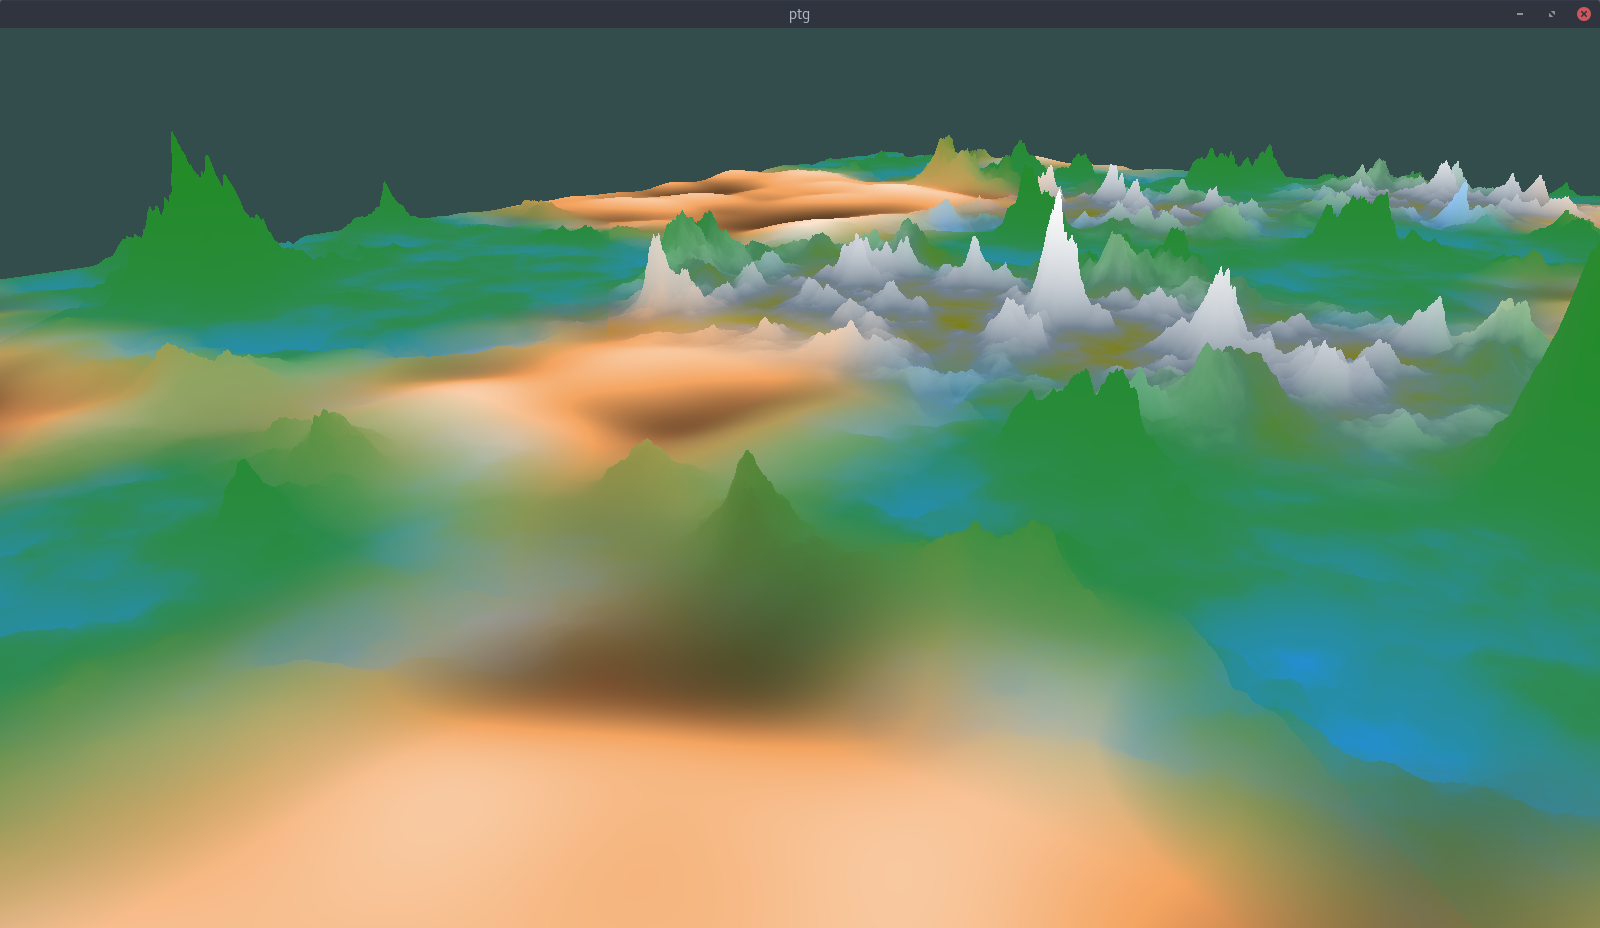
\includegraphics[width=0.48\textwidth]{figuras/resultados/l/resultSeed3Deltav05k2048b512l256.png}\label{fig:l256}}
%     
%     \caption{Alcance da fronteira.}
%     
%     \label{fig:lenghBioComp}
%     % usar \hspace{0.1cm}, é gambiarra mas funciona
%\end{figure}
%
%\begin{figure}[H]
%     \centering
%     \subfloat[][$seed = 1$]{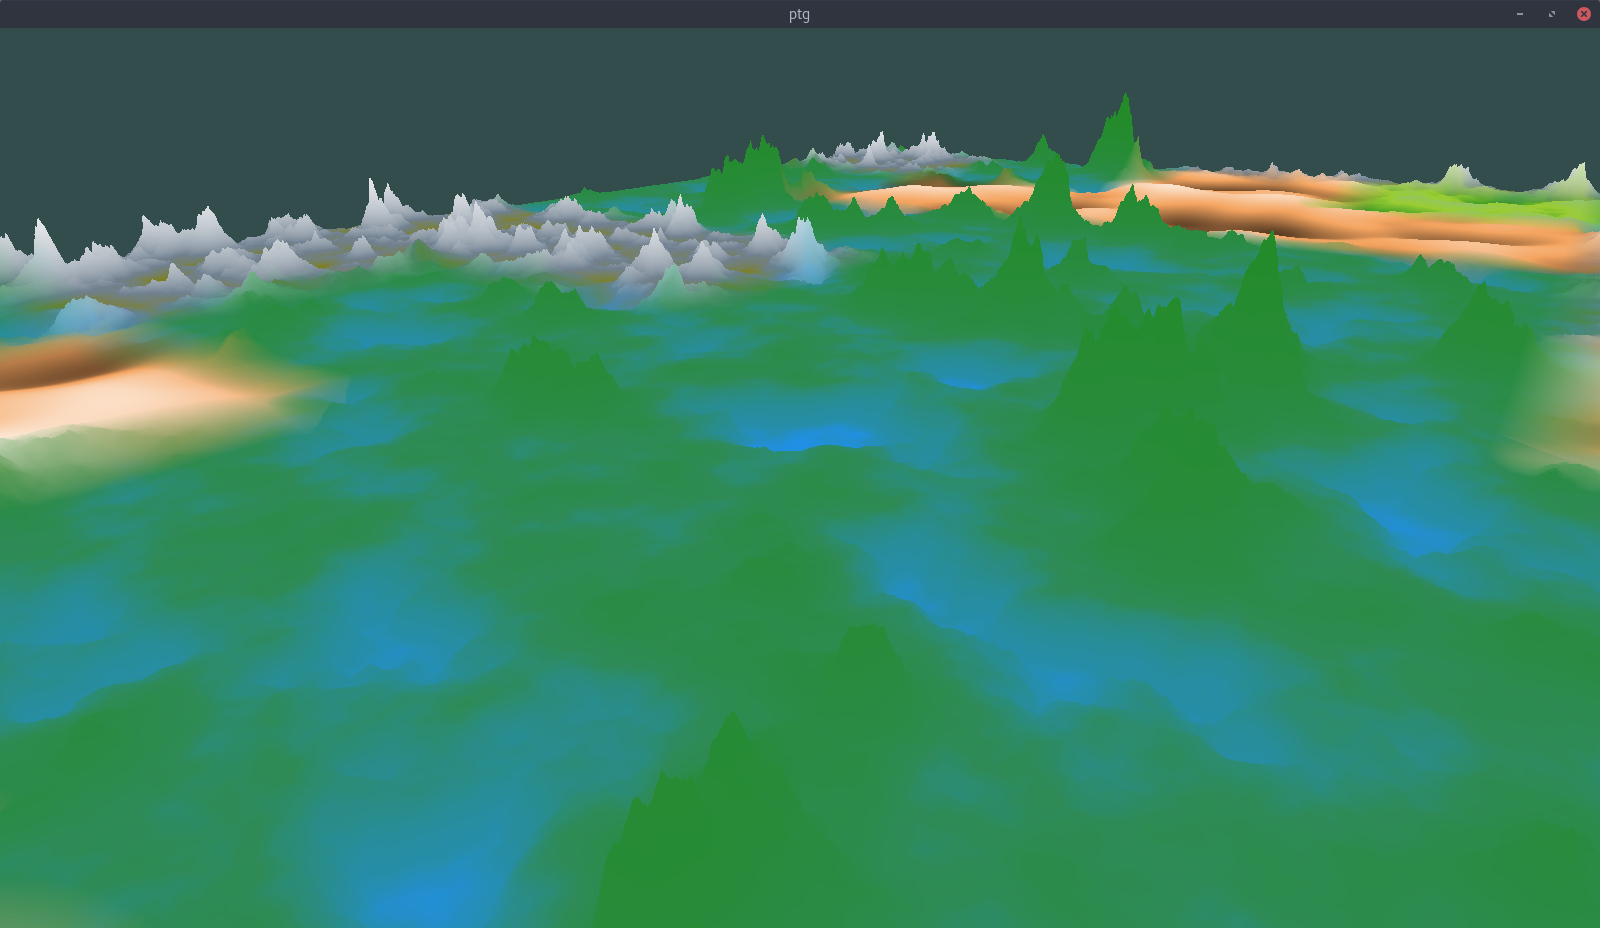
\includegraphics[width=0.48\textwidth]{figuras/resultados/seed/resultSeed1Deltav05k2048b512l128.png}\label{fig:bigseed1}}\hspace{0.1cm}
%     \subfloat[][$seed = 2$]{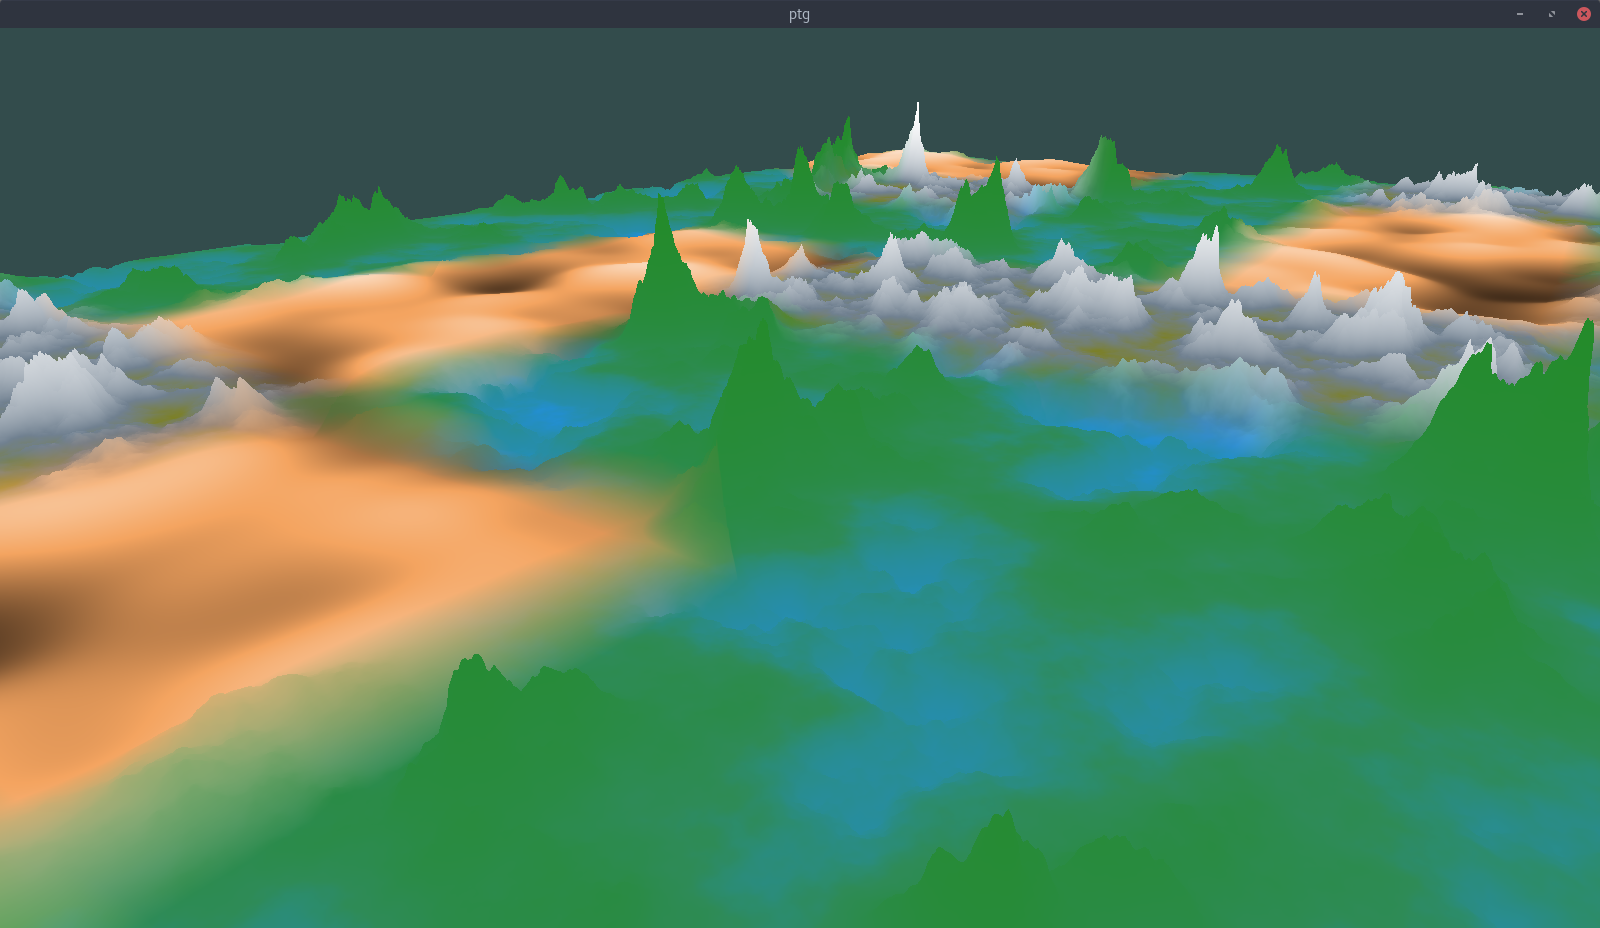
\includegraphics[width=0.48\textwidth]{figuras/resultados/seed/resultSeed2Deltav05k2048b512l128.png}\label{fig:bigseed2}}
%     
%     \caption{Semente para o motor de números pseudo aleatórios.}
%     
%     \label{fig:seedComp}
%     % usar \hspace{0.1cm}, é gambiarra mas funciona
%\end{figure}

%\begin{figure}[H]
%     \centering
%     \subfloat[][$fb = 2$]{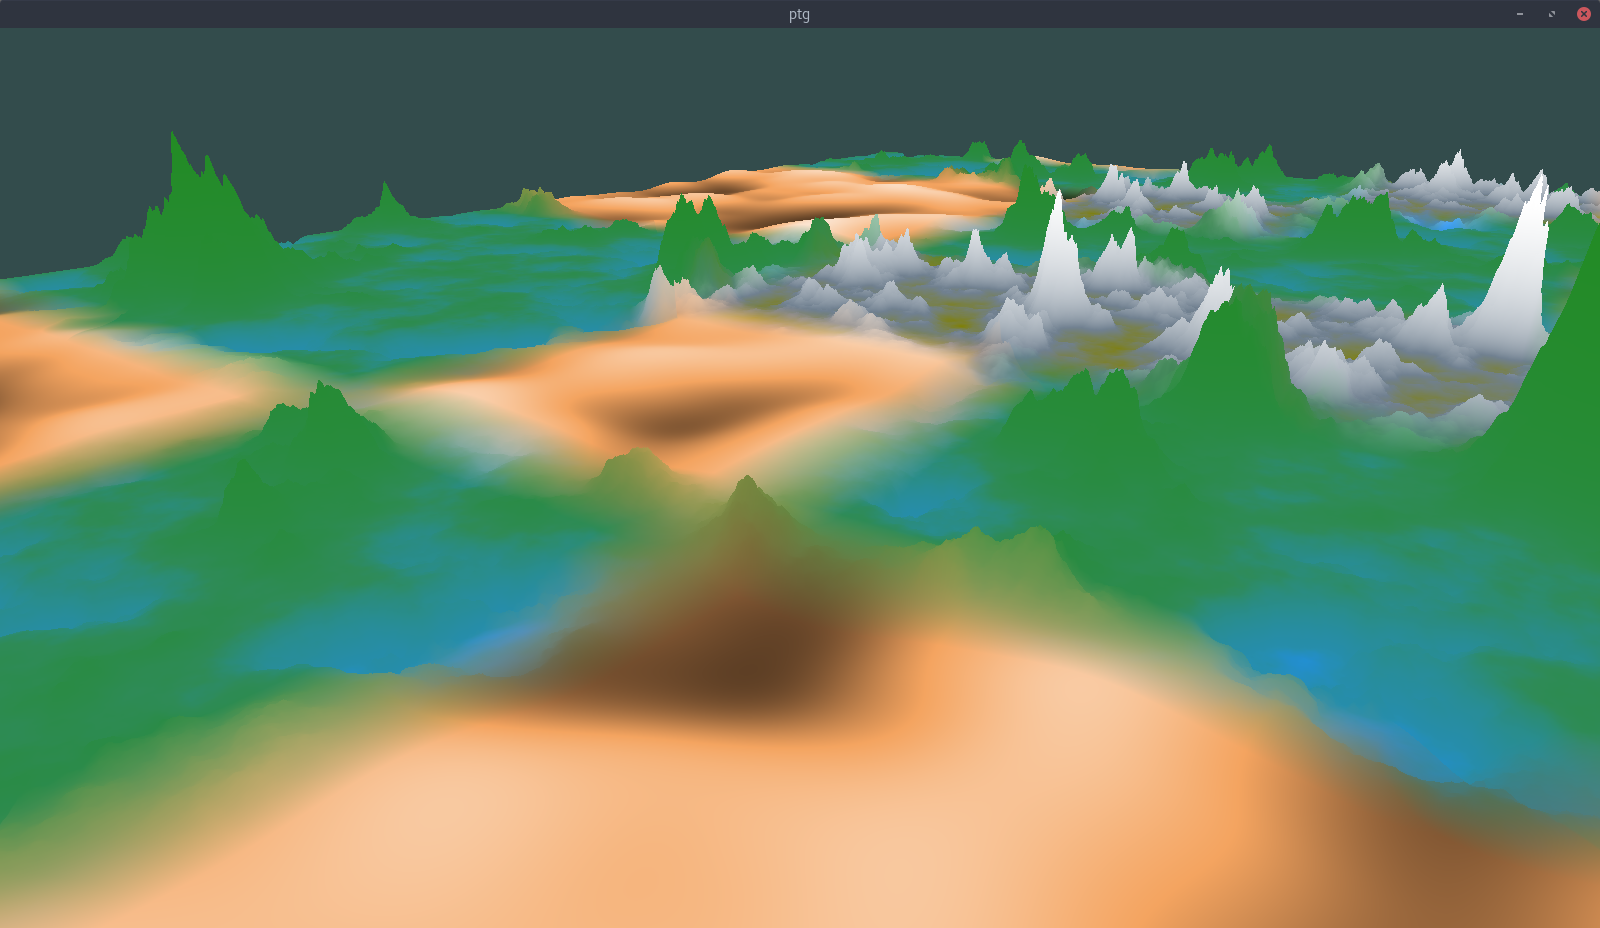
\includegraphics[width=0.48\textwidth]{figuras/resultados/freqb/resultSeed3Deltav05k2048b512l128freqb2.png}\label{fig:freqb2}}\hspace{0.1cm}
%     \subfloat[][$fb = 1/50$]{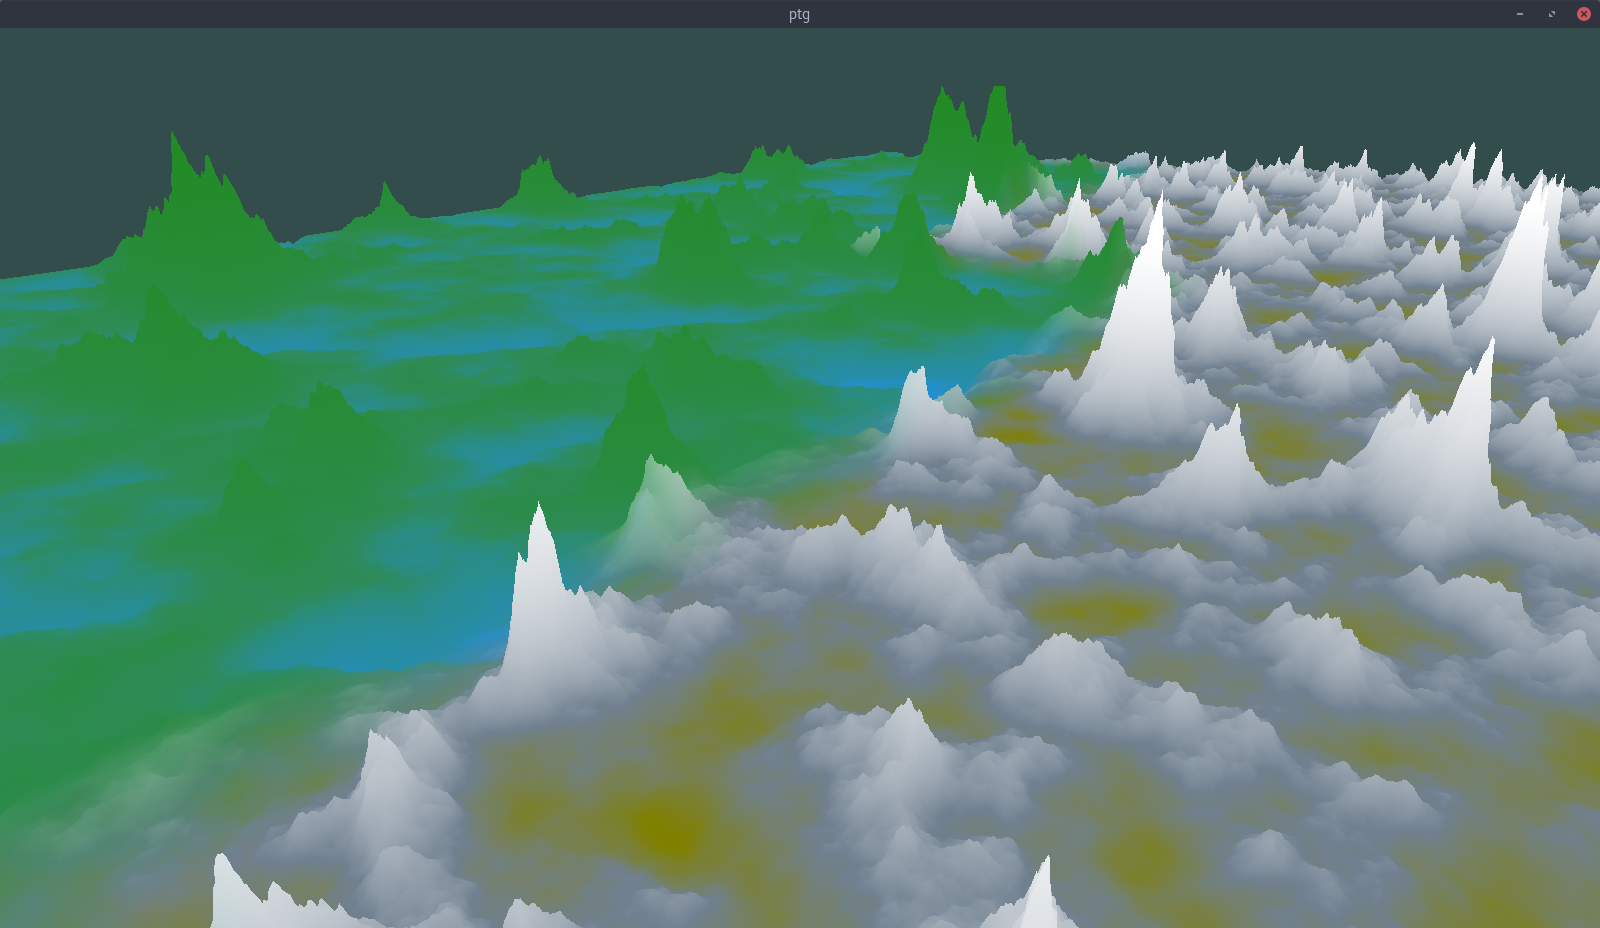
\includegraphics[width=0.48\textwidth]{figuras/resultados/freqb/resultSeed3Deltav05k2048b512l128freqb1_50.png}\label{fig:freqb1_50}}
%     
%     \caption{Frequência de biomas distintos.}
%     
%     \label{fig:freqbComp}
%     % usar \hspace{0.1cm}, é gambiarra mas funciona
%\end{figure}